\chapter{Hydro- and wind power}

Renewable energies are getting ever-increasing attention over the last decades. Worldwide investment in renewable technologies was $326.3$ billion US dollar in 2017 (the investment was peaked at 2017). Interestingly, China is the biggest investor in this sector, with almost a $50\%$ share. Globally, the predicted number of jobs is $7.7$ million associated with the renewable energy industry. Moreover, the systems are becoming more efficient and cheaper, and their share in total energy consumption is increasing. For instance, in 2019, more than two-thirds of worldwide newly installed electricity capacity was renewable.

The increasing attention has many factors. The most and widely known reason is the biggest challenge mankind has to face: global warming. Still, there are severe debates on how significant is the effect of the produced greenhouse gases (mostly $\mathrm{CO}_2$) by the globalized industry on the climate change, and how to act with our limited resources at our hand (prevent or adaptation). Another factor that gets less attention is the fact that the amount of fossil energy carriers are limited. Many researchers say that we are already passed the tipping point where a massive, long-lasting global economic crisis \textit{cannot} be avoided due to energy shortages. Simply, it is not possible to install renewable energy resources fast enough to avoid the shrinkage of the global economy. The third factor is an energy political question that is also a security issue; thus, it might be a less-known factor in common people. Fossil energy carriers are in great abundance only in a few countries, making the economy of the rest of the countries vulnerable. Since renewable energies are less focused by nature, the dependence can be reduced by investing in such technologies. Naturally, as we are living in a highly globalized world, unexpected events can significantly change the direction of our global history. For instance, an unexpected breakthrough of a new technology or the recent outbreak of the SARS-CoV-2 coronavirus might force us to redesign and develop a more energy-efficient, less vulnerable global economy. 

The discussion about renewable energies are always overheated, and opinions are mostly divided between two extremes. On the one hand, environmentalist says that renewable energies can cover all of our energy demand, we need only political will. On the other hand, many scientists claim that purely with renewable energy sources, the present consumption cannot be fully covered unless it is reduced significantly. Unfortunately, the arguments in the heated debates in the media are usually lack of numbers but filled with emotions. However, the question of energy balance between consumption and production is purely scientific; thus, an exact scientific answer can be given. In the following sections, two renewable energy sources are going to be discussed related to fluid dynamics: wind turbines and hydrodynamic power plants. Let the numbers speak for themselves.

% WIND TURBINES %%%%%%%%%%%%%%%%%%%%%%%%%%%%%%%%%%%%%%%%%%%%%%%%%%%%%%%%%%%%%%%
\section{Wind turbines}

In Chpt.\,\ref{chpt:fans}, the operation and behaviour of fans are discussed in details. They can be regarded as machines transforming electric energy as input to hydrodynamic energy (fluid flow) as output. Wind turbines behave in exactly the opposite way; they produce electricity from the kinetic energy of winds. Wind turbines consist of blades connected to a shaft that drives a generator. The whole system is strategically placed to catch the wind, which will then turn the blades and the shaft. The generator connected to the shaft will now produce electricity. The quality of the electricity generated from wind turbines is the same as those from other energy sources.

The size of wind turbines varies widely. The length of the blades is the most significant factor in determining the amount of electricity a wind turbine can generate. Small wind turbines that can power a single home may have an electricity generating capacity of $10\,\mathrm{kW}$. The most massive wind turbines in operation have electricity generating capacities of up to $10\,\mathrm{MW}$, and larger turbines are in development. Large turbines are often grouped to create wind power plants, or wind farms, that provide power to electricity grids.

%------------------------------------------------
\subsection{Classification of wind turbines}
There are two types of wind turbines: vertical axis wind turbines (VAWTs) and horizontal axis wind turbines (HAWTs). They both have their advantages and disadvantages. Horizontal-axis turbines have (usually three) blades like airplane propellers, where the rotating axis of the wind turbine is horizontal, or parallel with the ground, see the left-hand side of Fig.\,\ref{Fig:Examples_HAWT_VAWT}. The most massive horizontal-axis turbines are as tall as $110\,\mathrm{m}$ and have blades more than $30\,\mathrm{m}$ long. Taller turbines with longer blades generate more electricity due to the higher wind speed. Roughly speaking, doubling the height of the wind turbines, their power increases approximately by $30\%$. The advantage of HAWTs is their high power; that is, they can extract more electricity from a given amount of wind compared to VAWTs; because the rotating axis of the blades is parallel to the wind. Thus, horizontal axis wind turbines dominate the majority of the wind industry. In extensive wind application, horizontal axis wind turbines are almost all one will ever see. The disadvantage of the horizontal axis, however, is that it is generally heavier and it does not perform well in turbulent winds. Moreover, they require an additional yaw control mechanism to turn the blades toward the wind.

Vertical-axis turbines have blades that are attached to the top and the bottom of a vertical rotor; thus, the rotational axis of the turbine stands vertical or perpendicular to the ground. The most common type of vertical-axis turbine—the Darrieus wind turbine, named after the French engineer Georges Darrieus who patented the design in 1931, see the right-hand side of Fig.\,\ref{Fig:Examples_HAWT_VAWT}. Some versions of the vertical-axis turbine are $30\,\mathrm{m}$ tall and $15\,\mathrm{m}$ wide. Very few vertical-axis wind turbines are in use today because they do not perform as well as horizontal-axis turbines. One of the reasons is that for half the rotation time, the blades have to rotate against the wind. Due to this fact, vertical axis turbines are primarily used in small wind projects and residential applications. Their advantage in such small scale applications is the ability to be powered by the wind coming from all 360 degrees, and even some turbines are powered when the wind blows from top to bottom. Because of this versatility, vertical axis wind turbines are thought to be ideal for installations where wind conditions are not consistent, or due to public ordinances, the turbine cannot be placed high enough to benefit from steady wind.

\begin{figure}[ht!]
	\centering
		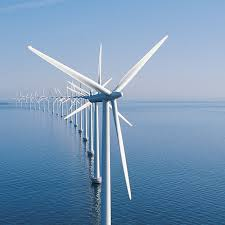
\includegraphics[height=6cm]{HydroAndWindPower/Figures/Example_HAWT.jpg}
		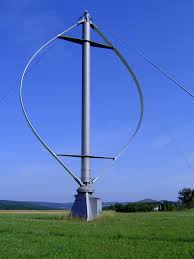
\includegraphics[height=6cm]{HydroAndWindPower/Figures/Example_VAWT.jpg}
	\caption{Typical examples of wind turbines. Left panel: horizontal axis wind turbine (HAWT). Right panel: Darrieus-type vertical axis wind turbine (VAWT).}
	\label{Fig:Examples_HAWT_VAWT}
\end{figure}

%------------------------------------------------
\subsection{Power and efficiency of horizontal axis wind turbines (HAWTs)} \label{power_and_efficiency_of_HAWTs}
In this section, the generated power and efficiency is discussed in details for horizontal axis wind turbine (HAWT), since these types used widely in large scale industrial applications. For this purpose, let us consider a streamtube around the wind turbine shown in Fig.\,\ref{Fig:SteamTube_HAWT} as a vertical cross-section. The boundary of the streamtube consists of sliding streamlines. Sliding means that velocity jump in the tangential direction can exist by crossing the streamline. For simplicity, let us replace the complex geometry of a wind turbine with a so-called actuator disc. The fluid (air) enters in the right-hand side of the streamtube (at cross-section $A_1$) with velocity $v_1$ that is equal to the undisturbed wind speed $v_{\infty}$. That is, at this cross-section, the velocity inside and outside of the streamtube is equal, see also the velocity distribution depicted by the arrows in Fig.\,\ref{Fig:SteamTube_HAWT}. In the streamtube, the fluid velocity slows down: at the cross-section of the actuator disc $A_2$, the velocity is $v_2<v_1$; and at the cross-section of the outlet $A_3$, the velocity is $v_3<v_2<v_1$. We assume that the inlet and outlet of the streamtube are relatively far away from the actuator disc; consequently, around the streamtube, the pressure is equal to the ambient pressure $p_0$. However, inside the streamtube, the pressure can change as the wind turbine produces a pressure difference between the two sides of the blades. That is, the pressure increases from $p_1$ to $p_2$ by crossing the actuator disc.

\begin{figure}[ht!]
	\centering
		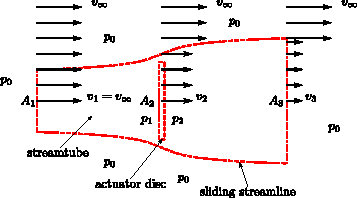
\includegraphics[height=6cm]{HydroAndWindPower/Figures/SteamTube_HAWT.pdf}
	\caption{Vertical cross-section of a streamtube around a horizontal axis wind turbine (HAWT). The actuator disc replaces the complex geometry of the wind turbine.}
	\label{Fig:SteamTube_HAWT}
\end{figure}

During the derivation of the useful power and efficiency of the wind turbine, the following assumptions are made. In a stationary co-ordinate system (compared to the wind turbine), the flow field is stationary. The fluid is assumed to be incompressible (the density $\rho$ is constant) and frictionless (the viscosity $\mu=0$). The gravitational force can be negligible. The axial velocity in a given cross-section is uniform and constant. Finally, the radial component of the flow velocity is zero.

As a first step, consider two Bernoulli equations. One between cross-sections $A_1$ and $A_2$:
%
\begin{equation} \label{bernoulli_1}
p_0 + \frac{\rho}{2} v_1^2 = p_1 + \frac{\rho}{2} v_2^2,
\end{equation}
%
and another one between cross-sections $A_2$ and $A_3$:
%
\begin{equation} \label{bernoulli_2}
p_2 + \frac{\rho}{2} v_2^2 = p_0 + \frac{\rho}{2} v_3^2.
\end{equation}
%
Keep in mind that a single Bernoulli equation between cross-sections $A_1$ and $A_3$ cannot be written as the streamlines are crossed (thus broken) by the blades of the wind turbine. With the help of Eqs.\,\eqref{bernoulli_1} and \eqref{bernoulli_2}, the force acting on the wind turbine can be expressed as
%
\begin{equation} \label{wind_turbine_force_from_bernoulli}
F = (p_1-p_2) A_2 = \frac{\rho}{2} (v_1^2-v_3^2) A_2 = \rho \frac{v_1+v_3}{2} (v_1-v_3) A_2.
\end{equation}

Now let us seek another equation for the force $F$. For the complex surface bounded by the red dashed lines in Fig.\,\ref{Fig:SteamTube_HAWT}, the macroscopic momentum balance in a general form reads as
%
\begin{equation} \label{macroscopic_momentum_balance_wind_turbines}
\frac{\partial}{\partial t} \int_V \left(\rho \underline{v} \right) dV + \int_A \rho \underline{v} \left( \underline{v} \cdot d\underline{A} \right) + \int_A p d\underline{A} = \int_V \rho \underline{g} dV.
\end{equation}
%
Since the fluid flow is assumed to be stationary, and the effect of gravity is neglected, Eq.\,\eqref{macroscopic_momentum_balance_wind_turbines} can be simplified to
%
\begin{equation} \label{macroscopic_momentum_balance_simplified1_wind_turbines}
\int_A \rho \underline{v} \left( \underline{v} \cdot d\underline{A} \right) + \int_A p d\underline{A} = 0.
\end{equation}
%
It is to be stressed, that the surface $A$ in the surface integrals in Eq.\,\eqref{macroscopic_momentum_balance_simplified1_wind_turbines} is composed by the surface of the stream tube (outer red dashed lines in Fig.\,\ref{Fig:SteamTube_HAWT}), and the bounding surface of the actuator disc (inner red dashed lines in Fig.\,\ref{Fig:SteamTube_HAWT}) as a solid body inside the fluid flow domain. The evaluation of the surface integral related to the pressure term is quite simple. The integral on the streamtube (outer red dashed line) is zero as the pressure is uniform with a value of $p_0$ at every point on the corresponding \textit{closed} surface. The integral on the complex geometry of the wind turbine represented by the actuator disc (inner red dashed lines) can be a cumbersome task; however, it is known that the pressure integral around a body yields the net force $F$ acting on that body (wind turbine here). Thus, Eq.\,\eqref{macroscopic_momentum_balance_simplified1_wind_turbines} becomes
%
\begin{equation} \label{macroscopic_momentum_balance_simplified2_wind_turbines}
\int_A \rho \underline{v} \left( \underline{v} \cdot d\underline{A} \right) + F = 0.
\end{equation}
%
As the velocity does not change significantly between the two sides of the actuator disc, the surface integral of the momentum is zero for the inner red dashed line in Fig.\,\ref{Fig:SteamTube_HAWT}. Moreover, as fluid crosses the streamtube only at cross-sections $A_1$ and $A_2$ with uniform and constant velocities, the final form of the macroscopic momentum balance is
%
\begin{equation} \label{macroscopic_momentum_balance_simplified3_wind_turbines}
-\rho v_1^2 A_1 + \rho v_3^2 A_3 + F = 0.
\end{equation}
%
The technique to integrate the macroscopic momentum balance on a given surface is already discussed in details in Sec.\,\ref{sec:pressure_amplitude_fast_closure}. With the aid of the conservation of mass (mass flow rate is constant at any given cross-section)
%
\begin{equation} \label{conservation_of_mass_wind_turbines}
\dot{m} = \rho v_1 A_1 = \rho v_2 A_2 = \rho v_3 A_3,
\end{equation}
%
the force acting on the wind turbine can be expresse from Eq.\,\ref{macroscopic_momentum_balance_simplified3_wind_turbines} as
%
\begin{equation} \label{wind_turbine_force_from_macroscopic_momentum_balance}
F = \rho v_1^2 A_1 - \rho v_3^2 A_3 = \rho v_2 A_2 (v_1 - v_3).
\end{equation}
%
By combinig Eqs.\,\eqref{wind_turbine_force_from_bernoulli} and \eqref{wind_turbine_force_from_macroscopic_momentum_balance}, the velocity at the actuator disc is
%
\begin{equation} \label{velocity_at_the_actuator_disc}
v_2 = \frac{v_1+v_3}{2},
\end{equation}
%
which is the mean value of the inflow $v_1$ and outflow $v_3$ velocities.

The useful power of a wind turbine is a hydraulic power:
%
\begin{equation} \label{useful_power_wind_power}
P_u = Q \Delta p = \frac{\dot{m}}{\rho} (p_1-p_2) = \frac{\dot{m}}{\rho} \frac{F}{A_2} = \frac{\rho v_2 A_2}{\rho} \frac{F}{A_2} = v_2 F,
\end{equation}
%
where $Q$ is the volume flow rate. Substituting Eqs.\,\eqref{velocity_at_the_actuator_disc} and \eqref{wind_turbine_force_from_macroscopic_momentum_balance} into Eq.\,\eqref{useful_power_wind_power}, and with some algebraic manipulation, the usful power becomes
%
\begin{equation} \label{useful_power_final}
P_u = \rho A_2 v_1^3 \left( 1 - \frac{v_1-v_3}{2 v_1} \right)^2 \frac{v_1-v_3}{v_1}.
\end{equation}
%
As a wind turbine transforms the kinetic energy of the wind into electric energy, the input power can be written as
%
\begin{equation} \label{input_power_wind_power}
P_i = \frac{1}{2} \dot{m} v_1^2 = \frac{1}{2} \rho A_2 v_1^3,
\end{equation}
%
calculating with the undisturbed velocity $v_1$ at the place of the actuator disc. That is, input power is obtained from the kinetic energy of the wind as if the wind turbine had not been there.

The efficiency of the wind turbine is simply the ratio of the useful and the input power:
%
\begin{equation} \label{efficiency_wind_power}
\eta = \frac{P_u}{P_i} = 2 \left( 1 - \frac{v_1-v_3}{2 v_1} \right)^2 \frac{v_1-v_3}{v_1} = 4 (1-x)^2 x,
\end{equation}
%
where
%
\begin{equation} \label{velocity_coefficient}
x = \frac{v_1-v_3}{2 v_1}.
\end{equation}
%
Interestingly, the efficiency has a global maximum as a function of $x$ that can be obtained by deriving Eq.\,\eqref{efficiency_wind_power} with respect to $x$, and find the root(s) of the resulted algebraic equation. The derivative is
%
\begin{equation}
\frac{\partial \eta}{\partial x} = 4 (1-x) (1-3x) = 0,
\end{equation}
%
whose solutions are $x_1=1$ and $x_2=1/3$. The frist root $x_1$ is a degenerate solution as it yields $v_3=-v_2$. Substituting the second root $x_2$ into Eq.\,\eqref{efficiency_wind_power}, the theoretical peak efficiency is
%
\begin{equation} \label{peak_efficiency_wind_power}
\eta_{max} = C_P^{max} = 4 (1-x_2)^2 x_2 = 0.593 \approx 60\%.
\end{equation}
%
Equation\,\eqref{peak_efficiency_wind_power} is quite expressive, as it states that only slightly more than half of the kinetic energy of the wind can be converted into hydrodynamics energy. Moreover, this hydrodynamics energy still has to be converted into electric energy via a generator reducing the overall efficiency further. The theoretical limit given by Eq.\,\eqref{peak_efficiency_wind_power} is called the Betz-limit. In many textbooks, the efficiency $\eta$ is referred to as the rotor power coefficient $C_P$. Substituting the value of $x_2$ into Eq.\,\eqref{velocity_coefficient}, it can be easily seen that at the best efficiency point, the outflow velocity is
%
\begin{equation}
v_3 = \frac{v_1}{3} = \frac{v_{\infty}}{3}.
\end{equation}
%
That is, in order to achieve peak performance, the wind turbine has to be designed (e.g., the profile of the blades) so that it slows the flow velocity down to $1/3$ of the undisturbed velocity $v_1=v_{\infty}$.

For a quick calculation, consider a well-designed wind turbine that can operate near the Betz-limit. Assume that the diameter of the turbine is $D=20\,\mathrm{m}$, the wind speed is $v_1=v_{\infty}=4\,\mathrm{m/s}$ and that the density of the air is $\rho=1.2\,\mathrm{kg/m^3}$. The useful power can be estimated as
%
\begin{equation}
P_u = P_i \cdot \eta_{max} = \frac{1}{2} \rho \frac{D^2 \pi}{4} v_{\infty}^3 \approx 7.1\,\mathrm{kW}.
\end{equation}
%
According to one of the reports of the World Energy Council, the average electric power consumption of a household in some countries in 2010 are as follows. United States: $11698\,\mathrm{kWh/year}=1.3\,\mathrm{kW}$, United Kingdom: $4648\,\mathrm{kWh/year}=0.53\,\mathrm{kW}$ and China: $1349\,\mathrm{kWh/year}=0.15\,\mathrm{kW}$. That is, a single installment of the wind power plant mentioned above can satisfy approximately the needs of $5.5$, $13.5$ and $47$ households, respectively. For more detailed calculations and conclusions, the reader is referred to Sec.\,\ref{design_aspects_and_further_remarks}.

%------------------------------------------------
\subsection{Design aspects and further remarks} \label{design_aspects_and_further_remarks}
The achievable useful power and maximum efficiency of a wind turbine depend on the design. Therefore, they can be determined only by measurements. By convention, the efficiency $\eta$ (rotor power coefficient $C_P$) is usually represented as a function of the tip speed ratio
%
\begin{equation} \label{tip_speed_ratio_wind_power}
\lambda = \frac{R \omega}{v_{\infty}},
\end{equation}
%
where $R$ is the radius of the turbine wheel, $\omega$ is its angular velocity and $v_{\infty}$ is the undisturbed wind speed. Observe that the term $R \omega$ is the circumferential velocity of the tip of the blades. Thus, Eq.\,\eqref{tip_speed_ratio_wind_power} is the ratio of the velocity of the fastest point in a blade and the undisturbed flow velocity. For different wind turbine designs, the characteristic curves are summarized in Fig.\,\ref{Fig:DesignPoint_HAWT_VAWT}. The Betz-limit is marked by the horizontal dashed line (ideal $C_P$). The theoretical power coefficient is shown by the green curve (infinite number of blades and lossless fluid flow). This curve initiates from the origin, and even with such an ideal case, the Betz-limit can be reached only above tip speed ratio approximately $\lambda=6$. Naturally, when the wind turbine stopped ($\lambda=0$), the efficiency is $\eta=C_P=0$ regardless of how carefully the wind turbine is designed. The other colour coded curves are measured characteristic curves of real wind turbine designs. They have a common feature; namely, there is an optimal tip speed ratio. It can be seen that the most efficient design is the three-bladed horizontal axis wind turbine, which justifies its exclusive usage in large-scale industrial projects.

\begin{figure}[ht!]
	\centering
		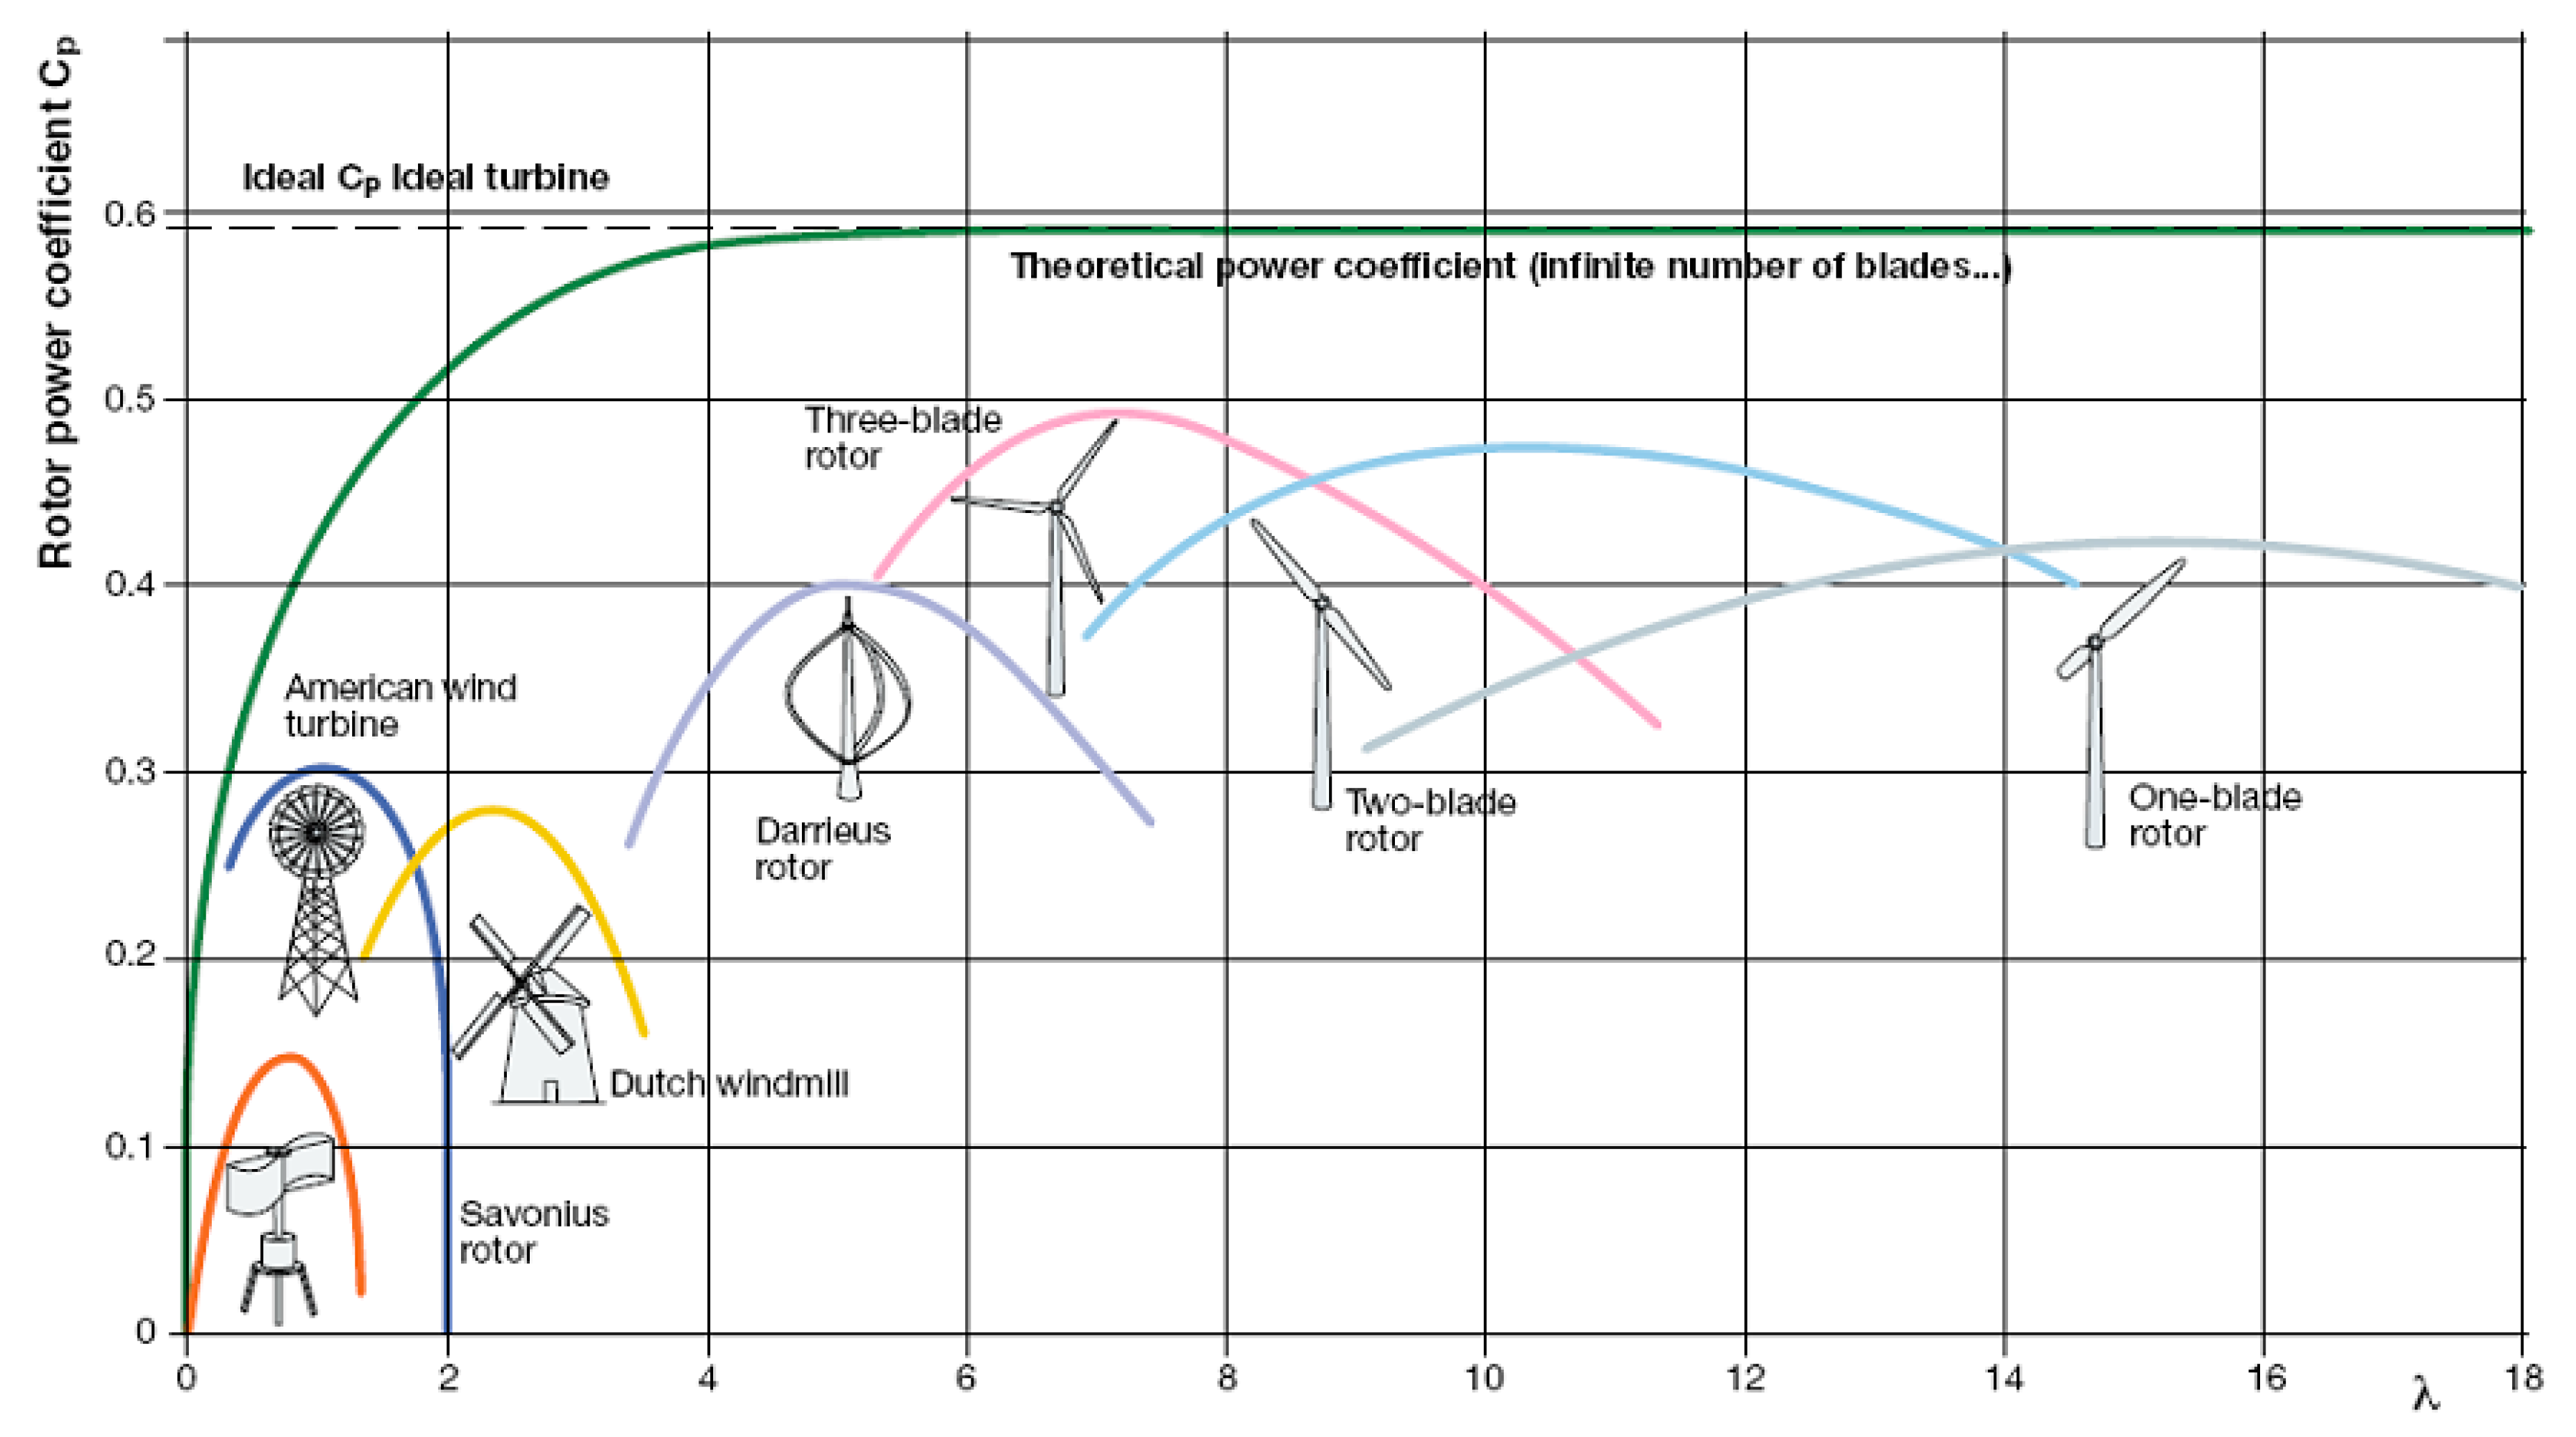
\includegraphics[height=8cm]{HydroAndWindPower/Figures/DesignPoint_HAWT_VAWT.png}
	\caption{Characteristic curves of different horizontal- and vertical axis wind turbines. The horizontal dashed line is the Betz-limit ($C_P=0.593$).}
	\label{Fig:DesignPoint_HAWT_VAWT}
\end{figure}

As a final remark, let us try to estimate the possible potential of the extensive installation of wind farms. Since the peak power of a single wind turbine is rather small (see the estimated calculation at the end of Sec.\,\ref{power_and_efficiency_of_HAWTs}), a massive number of wind turbines have to be put into operation in order to obtain a significant impact on the energy management. However, how much percentage of the territory of a country can be used for wind farms? Try to be realistic and assume $10\%$ that is actually a quite large number but still possible in theory. The next question is, how much power can be extracted in a unit area? Naturally, it depends on many factors; for instance, the average wind speed and how tightly the wind turbines are packed. Therefore, to obtain a good overview, use real data for an estimation: from the Whitelee wind farm near Glasgow in Scotland, see Fig.\,\ref{Fig:Whitelee_wind_farm}. The site area is $55\,\mathrm{km^2}$, the number of wind turbines is $215$, and the peak power is about $539\,\mathrm{MW}$. This means a peak power density of $9.8\,\mathrm{W/m^2}$. Naturally, a wind turbine cannot operate on their peak efficiency all the time. It is reasonable to assume (according to the experience) that a $30\%$ average load factor can be applied resulted in an approximated power density of $3\,\mathrm{W/m^2}$.

Continue the discussion with the United Kingdom as its wind energy potential is considered high. The population density of the country is approximately $255\,\mathrm{head/km^2}$ that translates to $4000\,\mathrm{m^2/head}$. Therefore, the electric power the wind farms can generate to a single person is approximately $1200\,\mathrm{W}=30\,\mathrm{kWh/day}$ (taking into account that ``only'' $10\%$ of the total land is used). In comparison, the used energy of an averaged driver in the United Kingdom is about $40\,\mathrm{kWh/day}$ (the list of assumptions and used data are omitted here to remained focused). Naturally, not every person are driving in the country; however, if one intends to use only electric cars, theoretically, the required power can barely be satisfied by installing wind turbines on $10\%$ of the landmass. Moreover, many other sectors are having a much bigger $\mathrm{CO}_2$ emission than domestic cars (e.g., heavy industry). In conclusion, there is a tremendous amount of wind power capacity worldwide; however, our consumption is also massive. The total wind power capacity in 2018 was $591\,\mathrm{GW}$, which is only $3.2\%$ of the total global energy consumption ($18394\,\mathrm{GW}$). Although the estimated peak wind power potential worldwide is $123\,\mathrm{PWh/y}=14031\,\mathrm{GW}$, the low power density ($3\,\mathrm{W/m^2}$) and the relatively short lifetime (5 years of offshore and 30 years of onshore wind turbines) will always be the primary limiting factor of the massive application of wind turbines. Nevertheless, they will play an ever-increasing role in the future, but the reduction of energy consumption or the exploitation of other renewable energy sources is a must (see the next section as an example).

\begin{figure}[ht!]
	\centering
		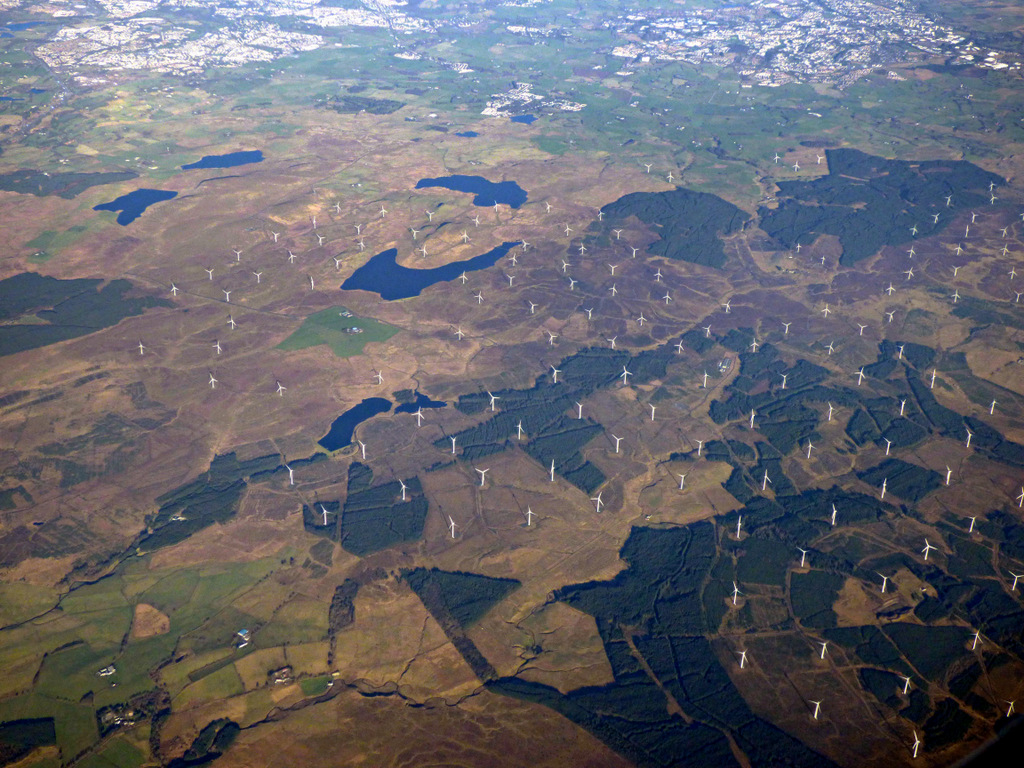
\includegraphics[height=8cm]{HydroAndWindPower/Figures/Whitelee_wind_farm_from_the_air.jpg}
	\caption{Whitelee wind farm from air and some of its $215$ wind turbines.}
	\label{Fig:Whitelee_wind_farm}
\end{figure}



% HYDROPOWER PLANTS %%%%%%%%%%%%%%%%%%%%%%%%%%%%%%%%%%%%%%%%%%%%%%%%%%%%%%%%%%%
\section{Hydropower plants}

Hydropower or water power is power derived from the energy of falling or fast-running water, which may be harnessed for useful purposes. That is, the potential energy and/or the kinetic energy of the water is utilised. In ancient times, hydropower from many kinds of watermills has been used as a renewable energy source for irrigation and the operation of various mechanical devices, such as gristmills, sawmills, textile mills, trip hammers, dock cranes, domestic lifts, and ore mills. In the late 19th century, hydropower began to used to produce electricity. The first such a power plant producing alternating current was built on the Niagara Falls in 1896 by Nikola Tesla and George Westinghouse. Interestingly, the first hydroelectric power plant in Europe was built in Serbia, also by Nikola Tesla, in 1900. Nowadays, the term hydropower has been used almost exclusively in conjunction with the modern development of hydroelectric power. Not long after the turn of the twenty-first century, hydropower development gained a renewed momentum. Between 2000 and 2017, nearly $500\,\mathrm{GW}$ in hydropower capacity was added worldwide (mainly across Asia and South America), representing an increase of $65\,\%$. The growth since 2010 has already outstripped what recorded in the first decade of the century. Today, hydropower provides about $16\,\%$ of the electricity of the world. According to the International Energy Agency, in order to meet the main energy-related components of the Sustainable Development Goals, including the below two degrees Celsius commitment of the Paris Agreement, an estimated $800\,\mathrm{GW}$ of additional hydropower will need to be brought online over the next two decades. Although hydropower is regarded as a clean and renewable energy source, it has several disadvantages as well, see Sec.\,\ref{introduction_to_hydropower} for details.

%------------------------------------------------
\subsection{Introduction to hydropower plants} \label{introduction_to_hydropower}
The type of hydropower plant suitable to build to a given place depends mainly on three factors.  The fist is the available water flow rate $Q$ and its fluctuation over seasons. The second is the available head $H$; that is, the possible static height difference of the water levels between the two sides of the power plant (representing the potential energy of the system). These two factors depend on the environment: local features of the landscape and the amount (and steadiness) of rainfall in the area of the drainage basin. With the help of the estimated values for average $Q$ and $H$, the theoretical (hydraulic, input) power and the produced electric (useful) power that can be harnessed from the power plant is
%
\begin{equation} \label{theoretical_power_hydropower}
P_{th} = P_{i} = Q \rho g H,
\end{equation}
%
and
\begin{equation} \label{electric_power_hydropower}
P_{el} = P_u = \eta_o P_{th} = \eta_o Q \rho g H,
\end{equation}
%
respectively. Here, $\eta_o$ is the total/overall efficiency of the instalment. The third factor is the flexibility in the power output. It depends both on the possibility of the hydropower plant itself and the requirements of the demand. In many cases, the variations in the demand can be satisfied by using large water reservoirs with which the peak power can be increased considerably for a limited amount of time.

The traditional type of hydropower plants is based on the installation of a dam that serves the purpose of elevating the available head $H$ and establishing a reservoir for storing a large amount of water supply. The schematic drawing of the operation is depicted in the top-left of Fig.\,\ref{Fig:traditional_hydropower_plants}. A dam is constructed across a river to elevate the water level and offer the fall needed to develop a driving force. The falling water is then channelled to a turbine wheel at a lower level. The flowing water turns a turbine wheel that is connected to a generator. The generator has a rotor, which is turned by the turbine. Finally, the turning of the generator rotor produces electricity. In the top-right panel of Fig.\,\ref{Fig:traditional_hydropower_plants}, the famous Hoover Dam (USA) is shown constructed between 1931 and 1936 (during the great depression). Its power capacity is $2080\,\mathrm{MW}$ that is not enough to be in the top 50 largest power plant in the world. The two largest hydropower plants are depicted in the bottom-left (Three Gorges Dam, China, $22500\,\mathrm{MW}$) and bottom-right (Itaipu Dam, border of  Brazil and Paraguay, $14000\,\mathrm{MW}$) panels of Fig.\,\ref{Fig:traditional_hydropower_plants}, respectively. In comparison, the peak power of the sole nuclear power plant in Hungary (Paks) has $2000\,\mathrm{MW}$ capacity.

\begin{figure}[ht!]
	\centering
		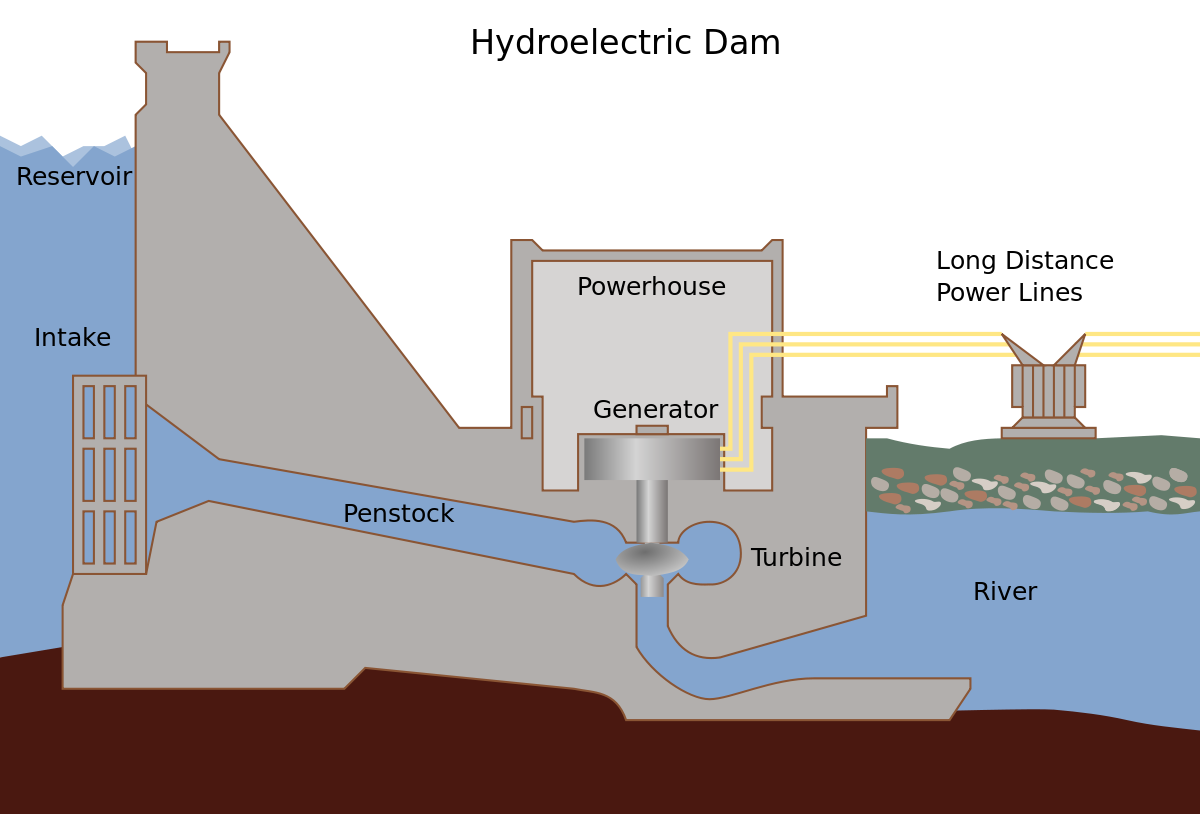
\includegraphics[width=6cm]{HydroAndWindPower/Figures/Schematics_Of_Traditional_Hydropower_Plants.png}
		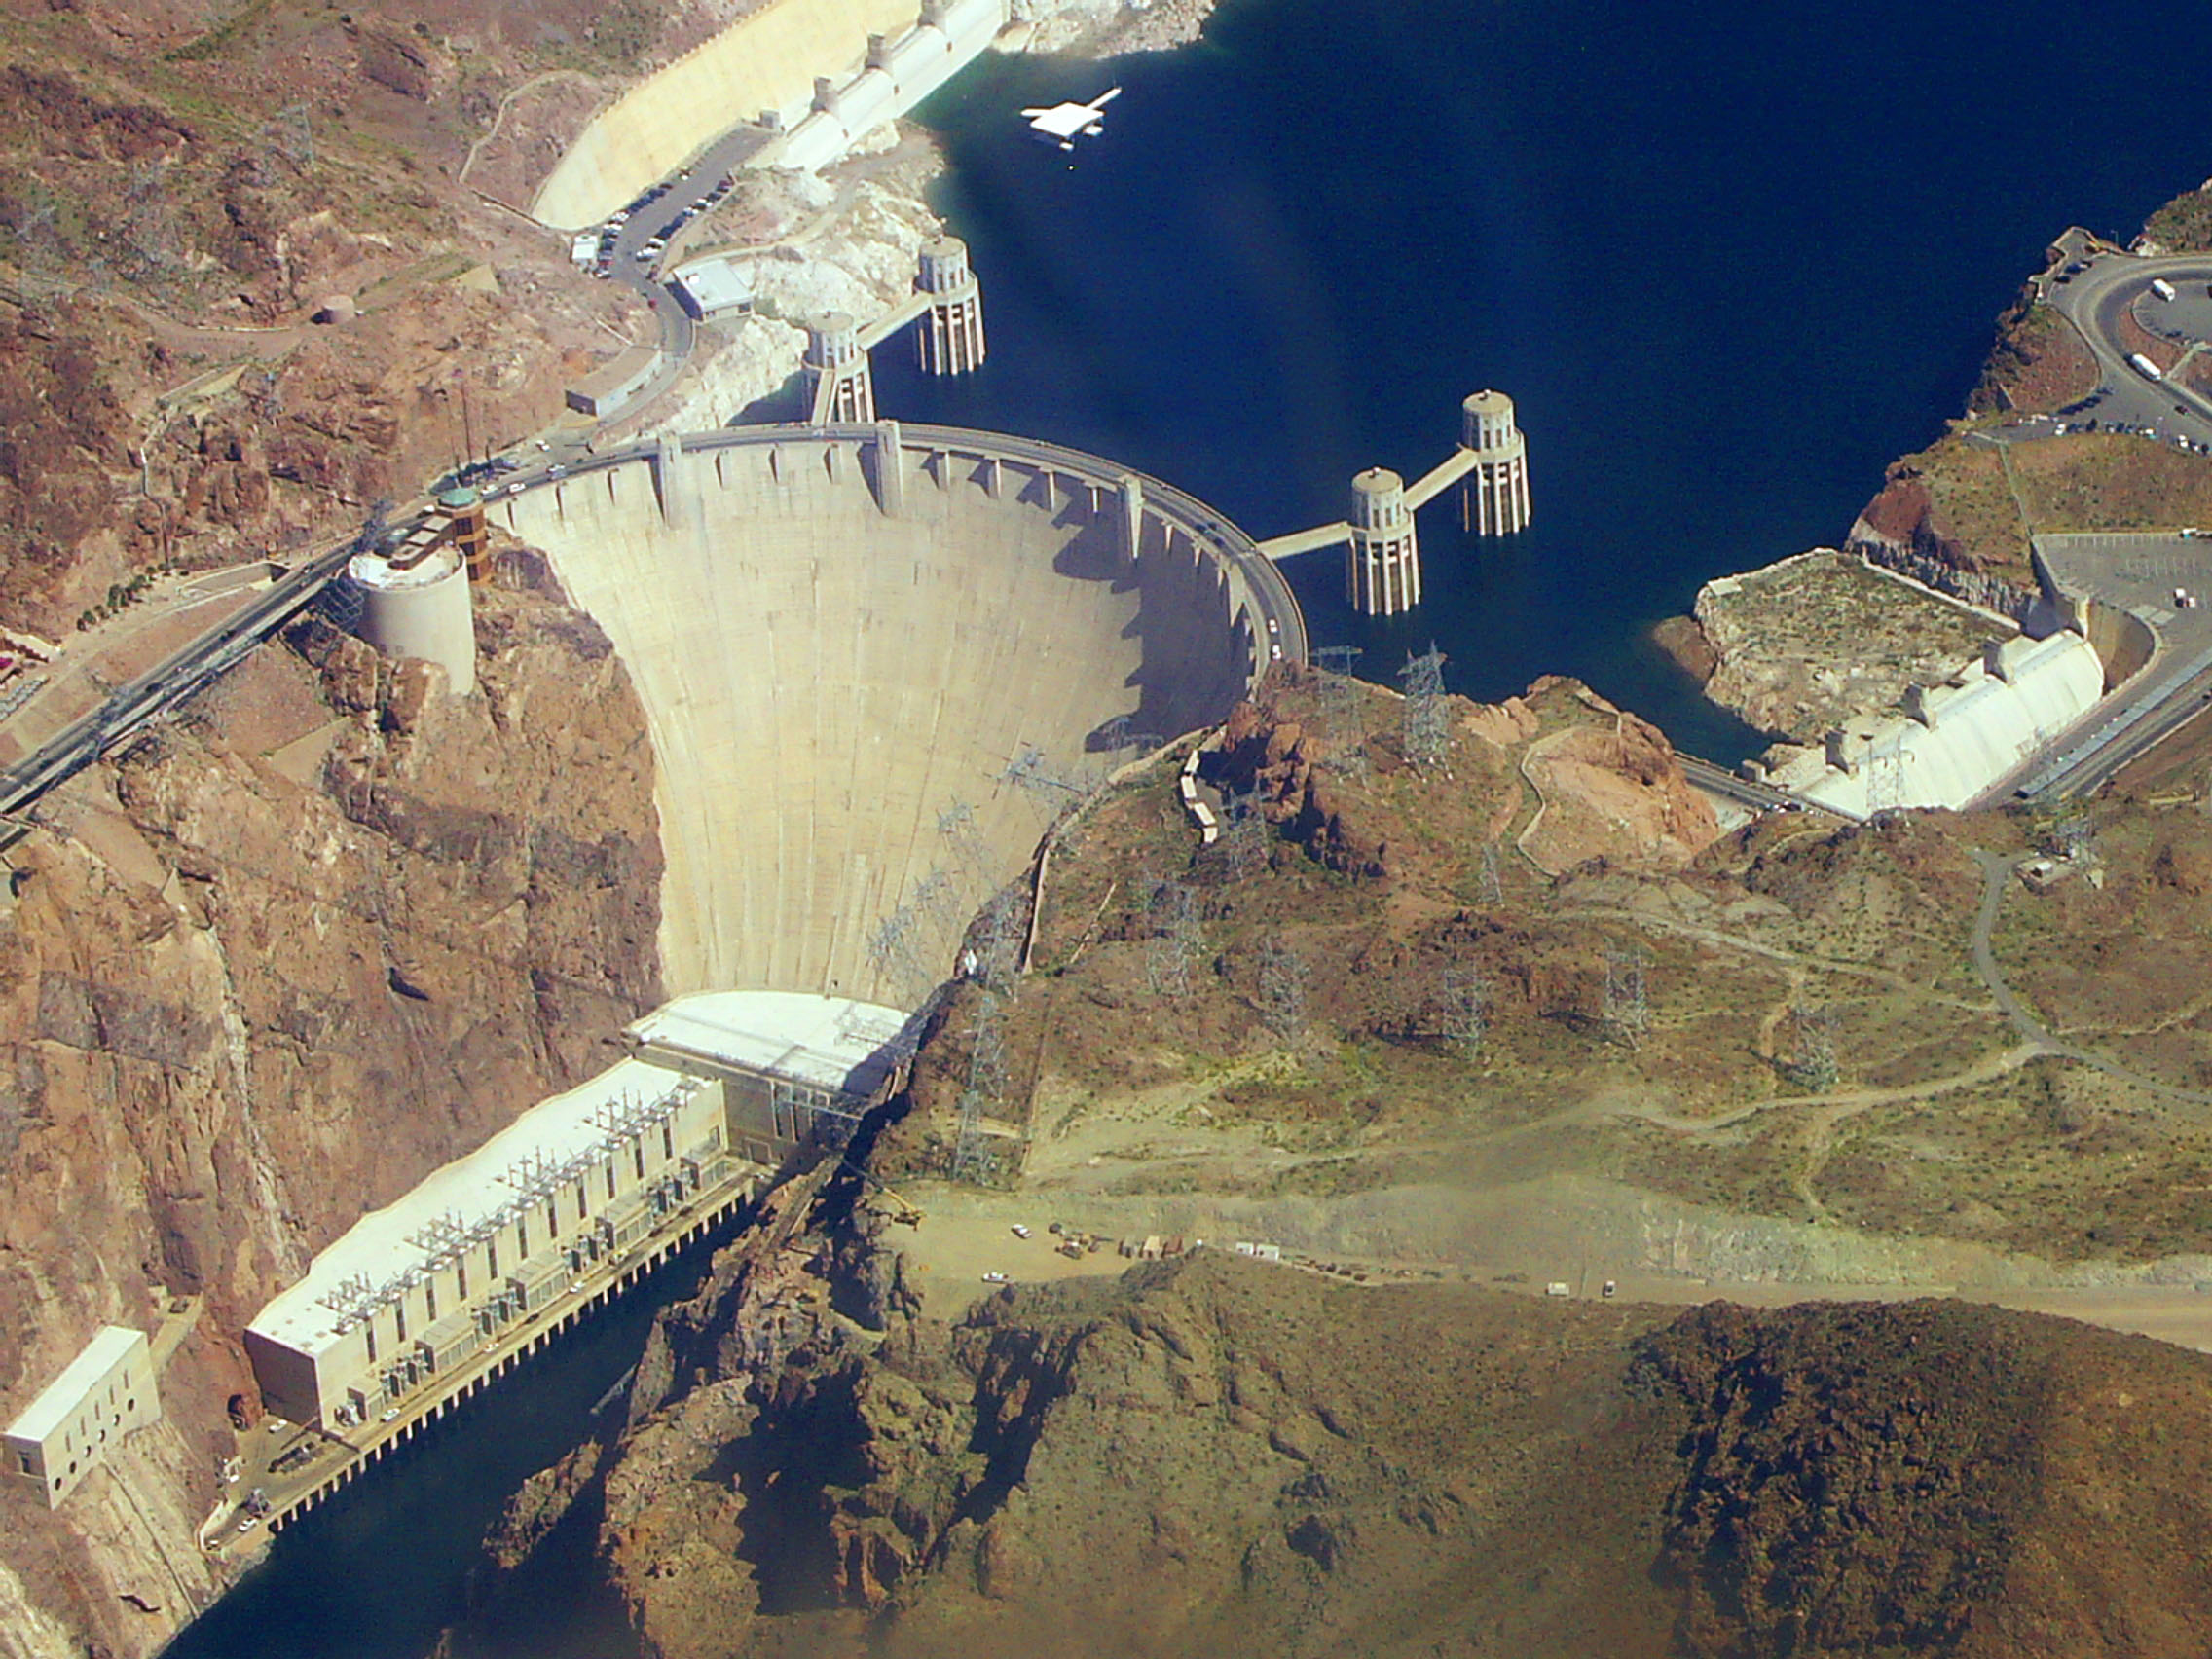
\includegraphics[width=6cm]{HydroAndWindPower/Figures/Hoover_Dam.jpg}
		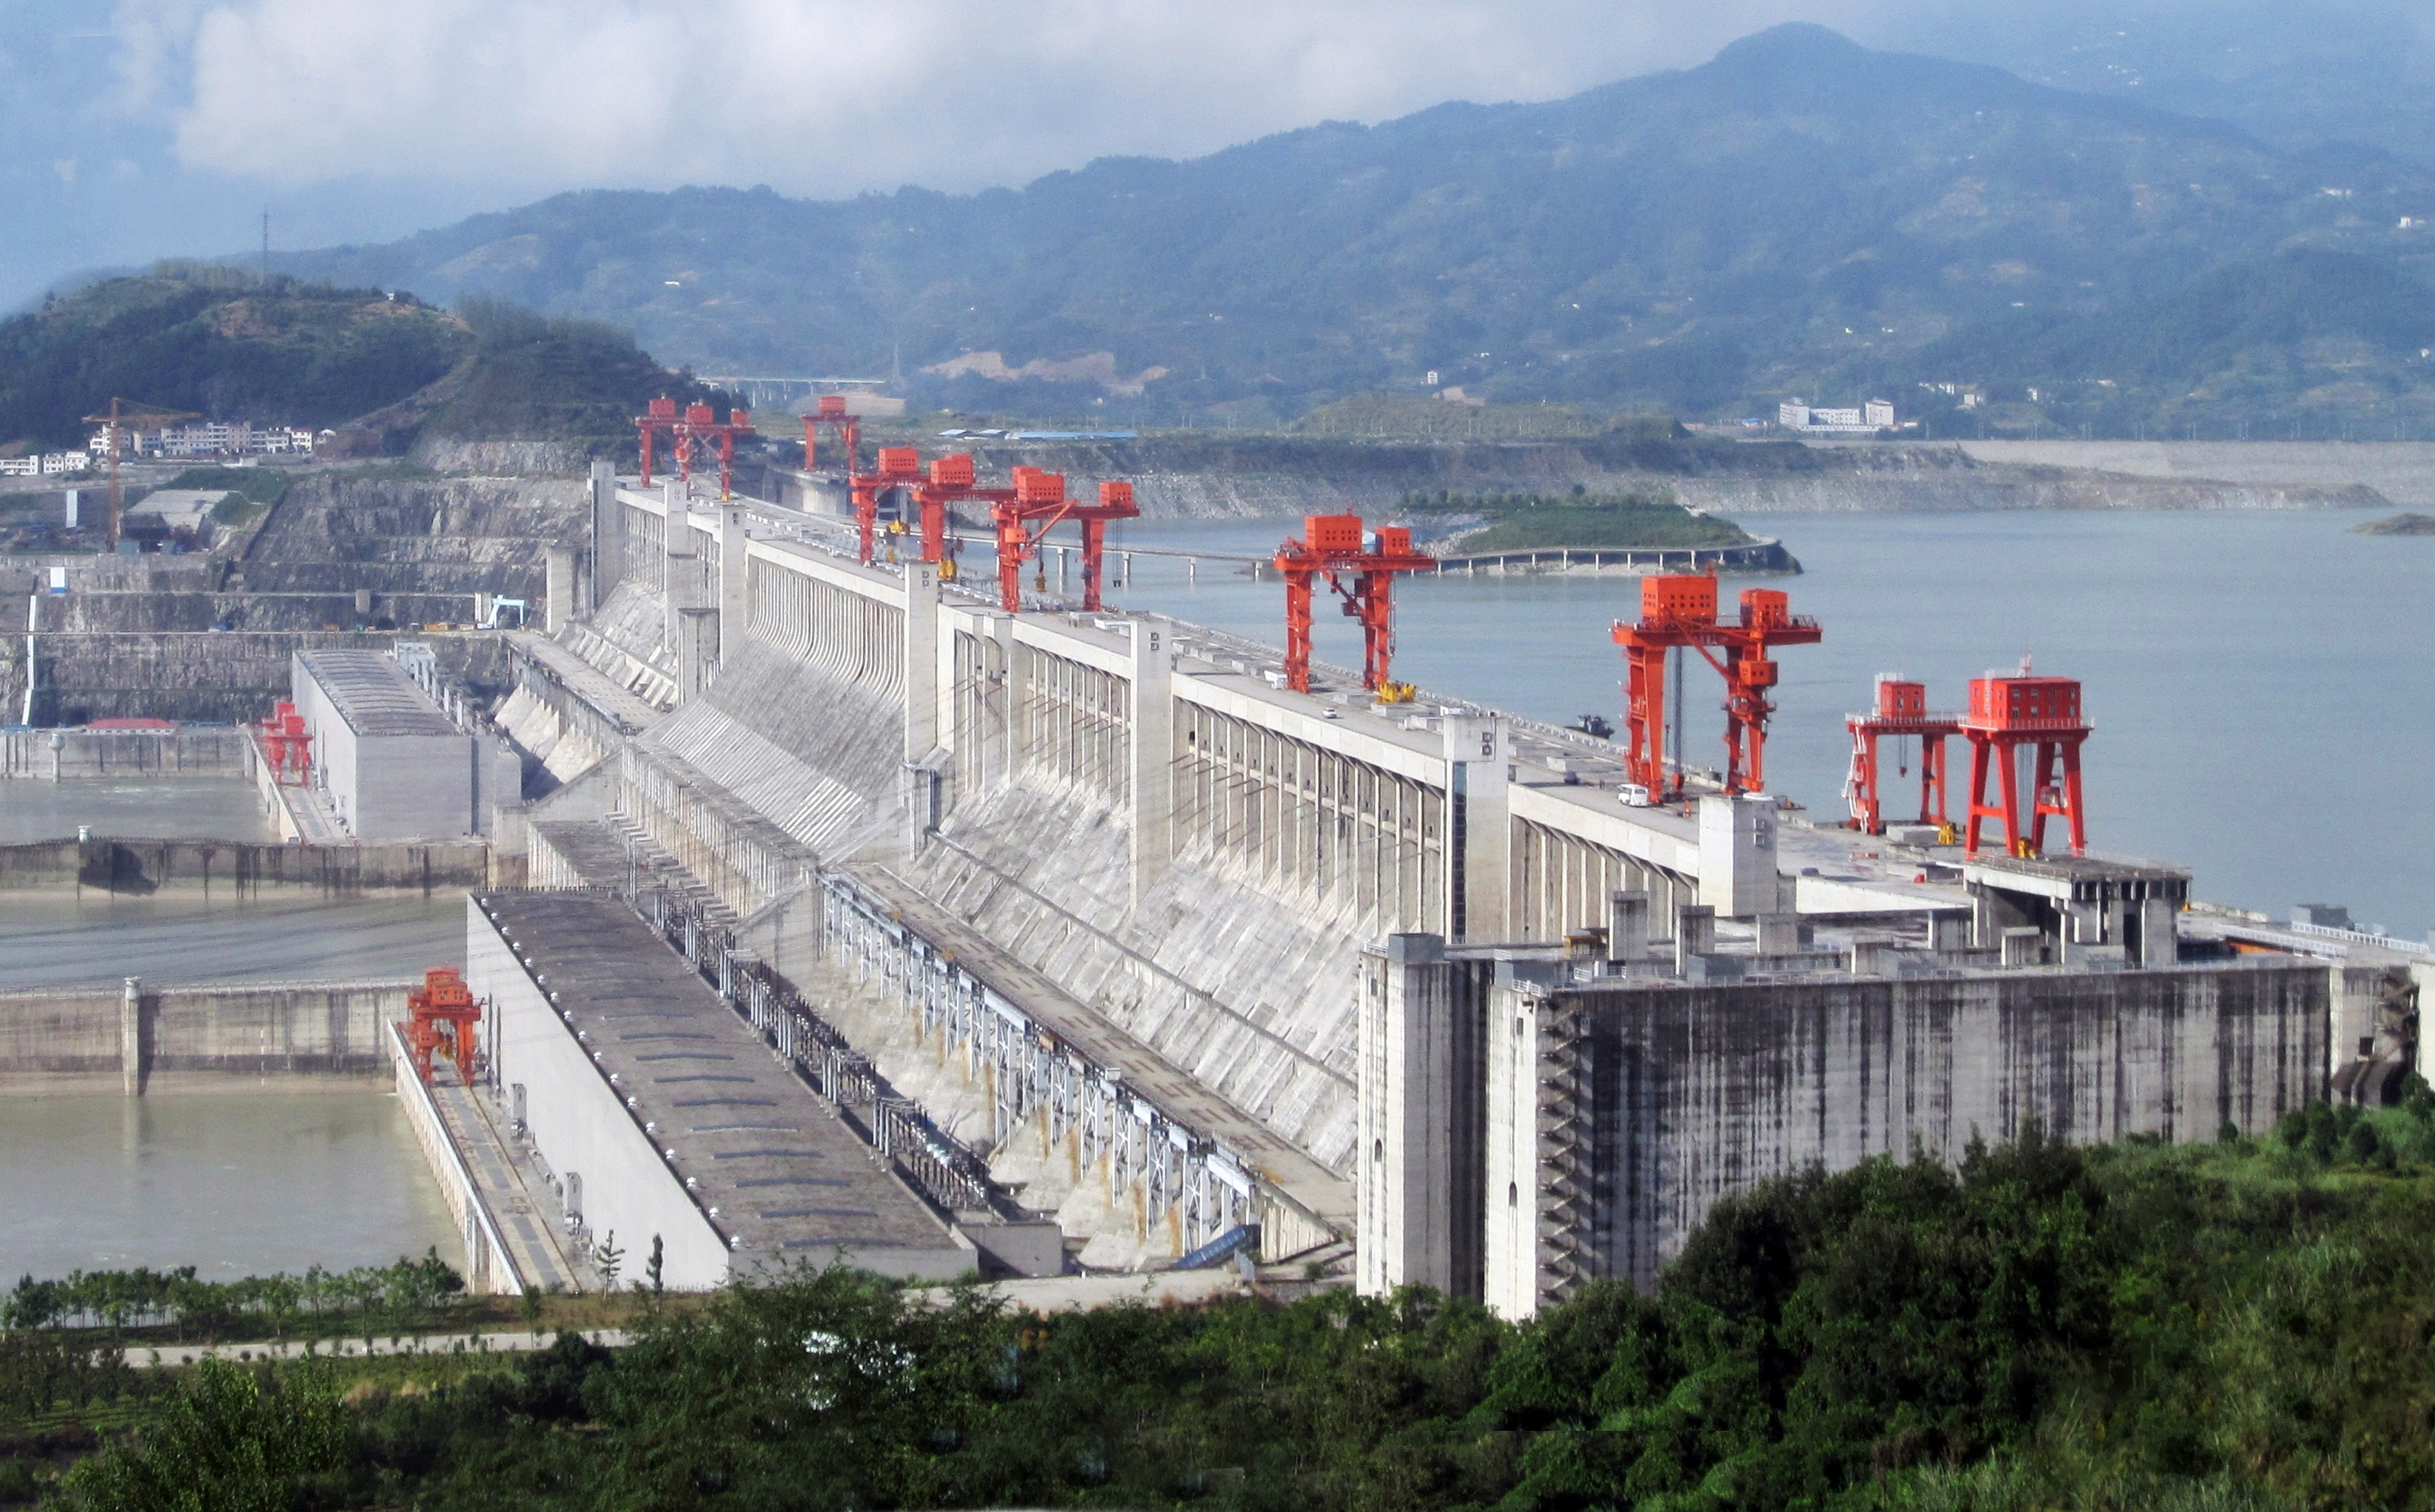
\includegraphics[width=6cm]{HydroAndWindPower/Figures/Three_Gorges_Dam.jpg}
		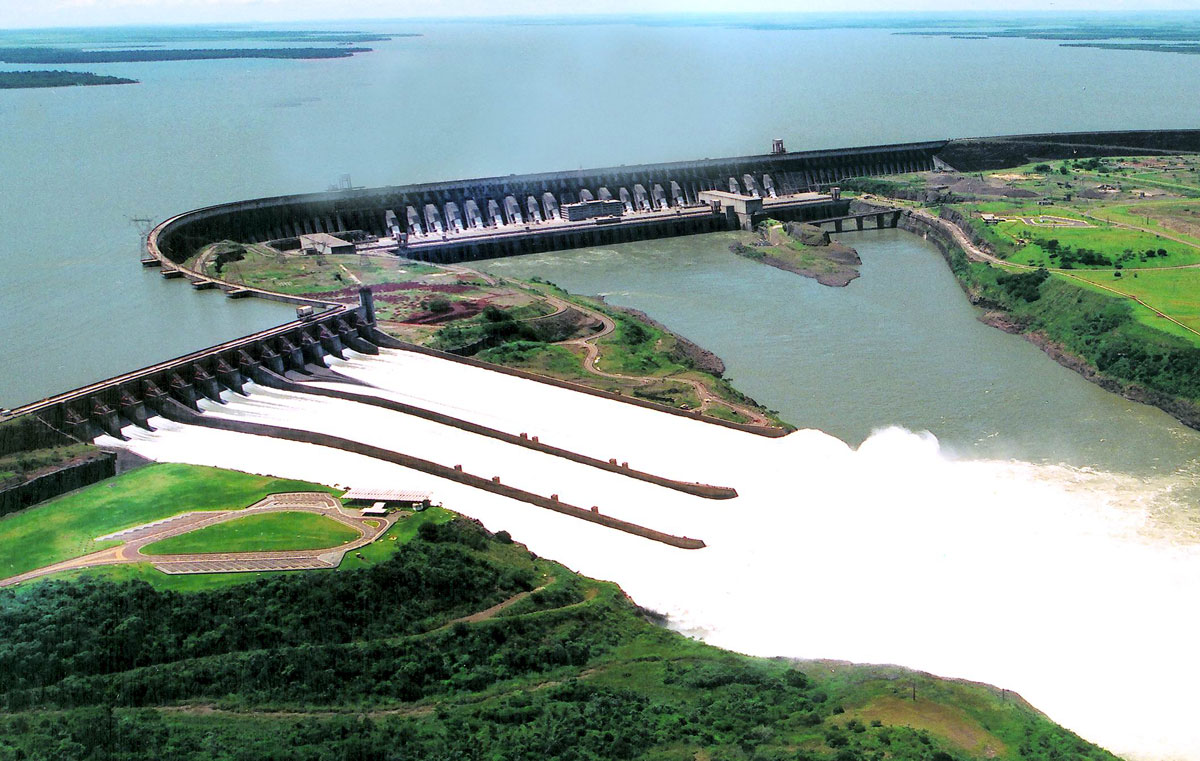
\includegraphics[width=6cm]{HydroAndWindPower/Figures/Itaipu_Dam.jpg}
	\caption{Tranditional (dam) hydropower plants. Top-left: schemtic draw of the operation; top-right: Hoover Dam, USA ($2080\,\mathrm{MW}$), bottom-left: Three Gorges Dam, China ($22500\,\mathrm{MW}$), bottom-right: Itaipu Dam, Brazil-Paraguay, ($14000\,\mathrm{MW}$).}
	\label{Fig:traditional_hydropower_plants}
\end{figure}

A special type of hydropower plant is the pumped-storage hydroelectricity or pump-turbine system. The main purpose of this system is to store energy (as the potential energy of the stored water) in an artificial reservoir at an elevated height. The storing process takes place usually in a period of low-cost electricity. During the high demand for electricity, the stored water is released through turbines to produce electric power. The schematic drawing of the operation is depicted in the left-hand side of Fig.\,\ref{Fig:pumped_storage_hydropower}. If the pumped-storage system is not connected to a traditional hydropower plant or the turbines does not feed by a river; that is, if the only aim is to compensate the daily fluctuations in the demand, the power plant is a net energy consumer. To date, there is no cheap and efficient technology to store a large amount of electric power; therefore, such systems play an important role to ``collect'' energies that would be wasted otherwise. For instance, the solar, wind and other renewable sources; in addition, the excess electricity from continuous base-load sources (e.g., coal or nuclear) to be saved for periods of higher demand. Pumped storage is by far the largest-capacity form of grid energy storage available. As a limitation, the capacity of the artificial reservoir is small, which can store enough water usually for less than half a day. The main reason is the specialised site required: both geographical height and water availability are necessary. These areas customarily have outstanding natural beauty, and therefore there are also social and ecological issues to overcome. The average energy efficiency of pumped-storage hydropower plants varies between $70\%–80\%$, in some exceptional cases, it can be as high as $87\%$. In the right-hand side of Fig.\,\ref{Fig:pumped_storage_hydropower} the Kinzua Dam is shown from a downriver view together with the Seneca Pumped Storage Generating Station (upper artificial reservoir). The storage capacity of the instalment is $3920\,\mathrm{MWh}$ with storage of $11.2\,\mathrm{h}$. Its peak power is about $390\,\mathrm{MW}$.

\begin{figure}[ht!]
	\centering
		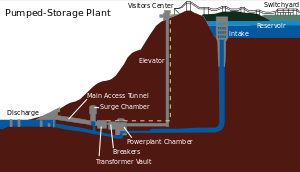
\includegraphics[width=6cm]{HydroAndWindPower/Figures/Schematics_Of_Pumped_Storage_Hydroelectricity.png}
		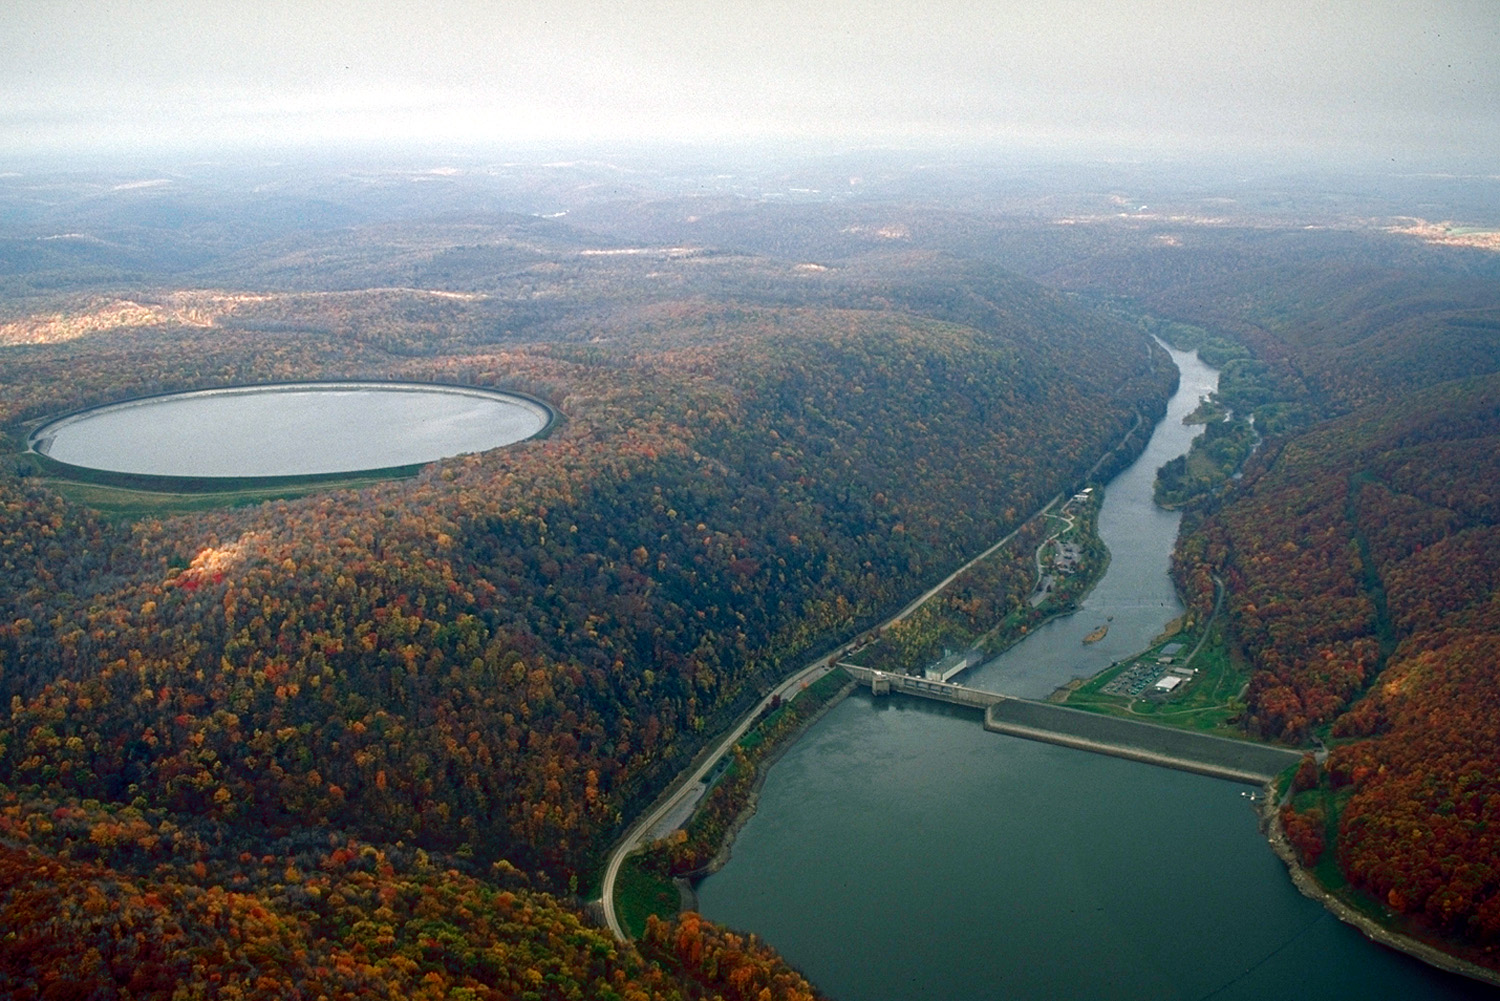
\includegraphics[width=6cm]{HydroAndWindPower/Figures/Kinzua_Dam.jpg}
	\caption{Pumped-storage hydroelectricity or pump-turbine system. Left: schematic draw of the operation; right: Kinzua Dam with the Seneca Pumped Storage Generating Station (upper artificial reservoir), USA ($3920\,\mathrm{MWh}$, $11.2\,\mathrm{h}$).}
	\label{Fig:pumped_storage_hydropower}
\end{figure}

If the landscape of the area does not allow to build a large dam (e.g., due to large flat habitable, agricultural or industrial regions), low head (below $15-5\,\mathrm{m}$) hydropower generation is the only option to produce electricity, where a little or no water storage is available. Many textbooks also refer to these power plants as run-of-river hydroelectricity. For the schematic drawing of the operation, see the left-hand side of Fig.\,\ref{Fig:low_head_hydropower}. In some cases, there is also a small storage reservoir called pondage. A plant without pondage is subject to seasonal river flows; thus, the plant will operate as an intermittent energy source. Naturally, low head hydropower plants have much less capacity as the traditional dam-type versions. However, they have many advantages. For instance, they still can be economically feasible, and like most hydro technologies, the output is predictable; therefore, it is a reliable renewable resource for electricity generation. In many cases, low head hydro generation can be added where low head dams and other hydraulic structures already exist for flood control, irrigation, and water regulation. It requires a smaller impounded area than large hydro projects and therefore has a less environmental impact and investment costs (smaller structures). It can greatly help to increase the use of clean power, particularly in remote locations where diesel generation is currently the primary source of electricity. In the right-hand side of Fig.\,\ref{Fig:low_head_hydropower}, the low-head hydropower plant at Tiszal\"ok is depicted (Hungary). Its peak power is approximately $11.5\,\mathrm{MW}$ with head about $7\,\mathrm{m}$. 

\begin{figure}[ht!]
	\centering
		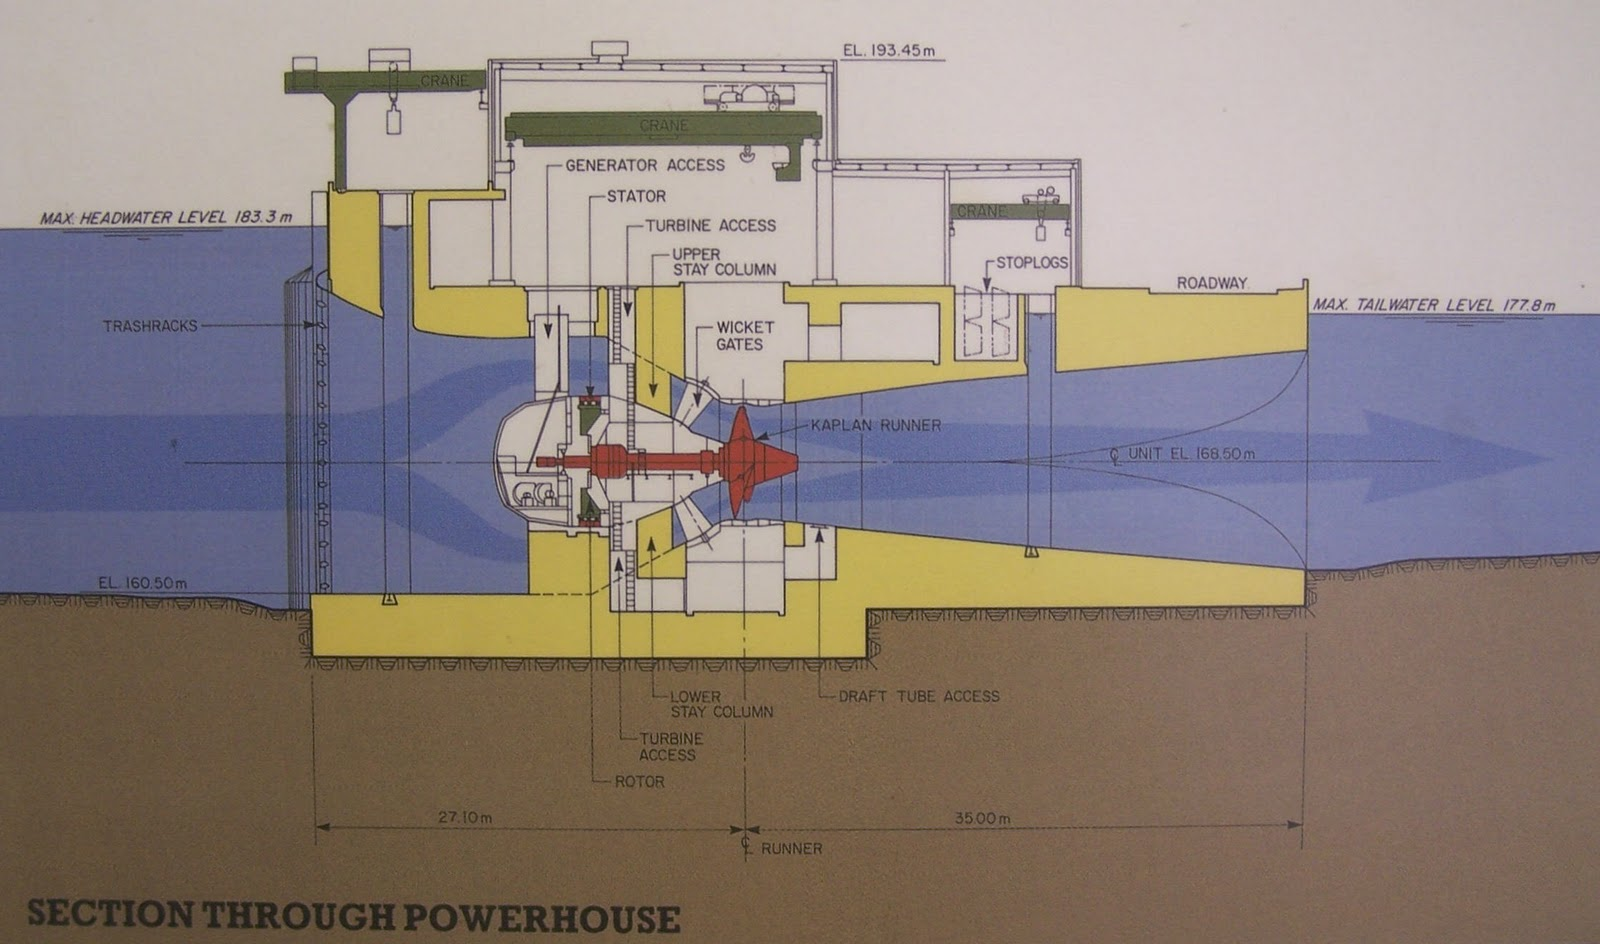
\includegraphics[height=4cm]{HydroAndWindPower/Figures/Shematics_Of_Low_Head_Hydropower.jpg}
		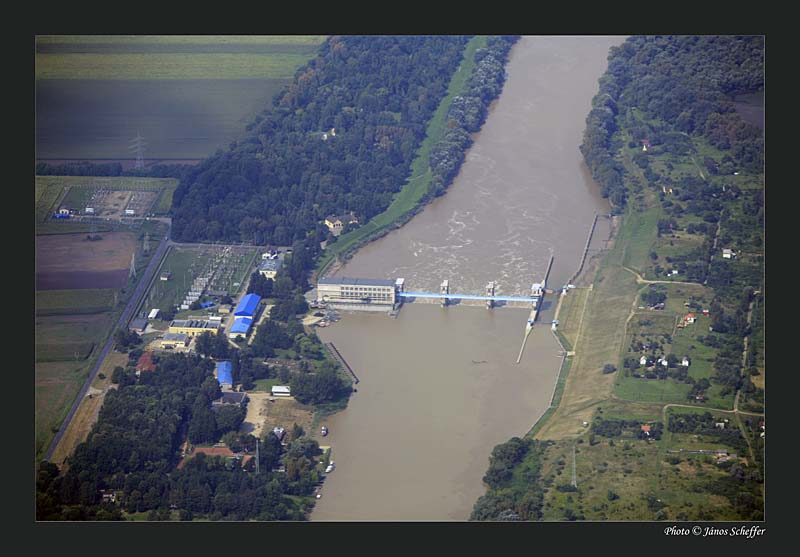
\includegraphics[height=4cm]{HydroAndWindPower/Figures/Tiszalok_Low_Head_Hydropower.jpg}
	\caption{Low head hydropower plants. Left: schematic draw of the operation; right: Tiszal\"ok low-head hydropower plant, Hungary ($11.5\,\mathrm{MW}$ peak power, $7\,\mathrm{m}$ head).}
	\label{Fig:low_head_hydropower}
\end{figure}

As the last example, tidal energy also has the potential for electricity generation, although they are still not widely used. Like all the other hydropower sources, electricity generation is more predictable compared to other renewable energy sources, e.g., wind and sun. Tidal energy has traditionally suffered from relatively high cost and limited availability of sites with sufficiently high tidal ranges or flow velocities; thus, constricting its total availability. However, many recent technological developments and improvements, both in design (e.g., dynamic tidal power, tidal lagoons) and turbine technology (e.g., new axial turbines, cross-flow turbines), indicate that the total availability of tidal power may be much higher than previously assumed and that economic and environmental costs may be brought down to competitive levels. In Fig.\,\ref{Fig:tidal_hydropower}, the schematic drawing of a tidal hydropower farm (left) and a real tidal power generator in Northern Ireland with a capacity of $1.2\,\mathrm{MW}$ (right) is depicted.

\begin{figure}[ht!]
	\centering
		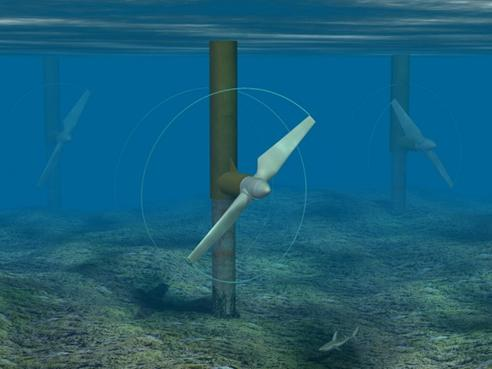
\includegraphics[height=4cm]{HydroAndWindPower/Figures/Schematics_Of_Tidal_Hydropower.jpg}
		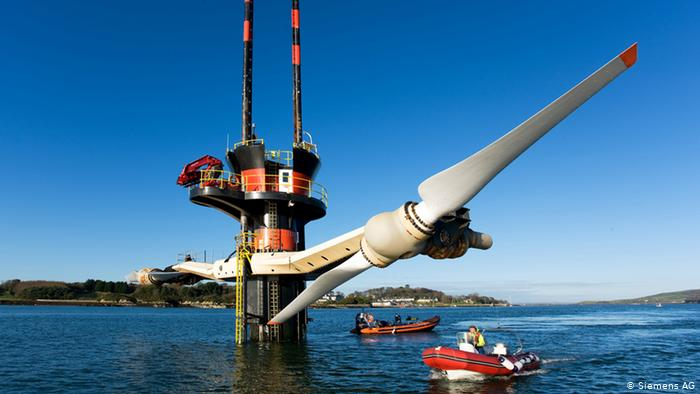
\includegraphics[height=4cm]{HydroAndWindPower/Figures/Tidal_Hydropower_In_Northen_Ireland.jpg}
	\caption{Tidal hydropower plants. Left: schematic draw of a tidal hydropower farm; right: a tidal power generator in Northern Ireland ($1.2\,\mathrm{MW}$).}
	\label{Fig:tidal_hydropower}
\end{figure}

After summarizing the types and constructions of hydropower plants, let us discuss their advantages and disadvantages. First of all, hydropower is a renewable energy source like rivers, and lakes typical never disappear. On the other hand, there are just a few suitable repositories where hydroelectric power plants could be built and fewer places where such undertakings are beneficial. In addition, hydroelectric power is a ``green'' and ``clean'' energy sources; they do not produce any toxic or greenhouse gases that pollute the atmosphere. The primary contamination happens when the power plants are being built. Hydroelectric power is a cost-competitive source of energy even though the upfront building costs can be high. River water is an infinite and reliable, long-lasting and constant resource, which is not affected by market volatility. Hydroelectric power plants have an average lifetime of 50–100 years, meaning they are strategic investments that can support many future generations. They can also be easily upgraded with novel technologies resulting in considerably lower operating and maintenance costs. The lake that forms behind the dam can be used for irrigation purposes, and it shields water tables from exhaustion and minimizes our susceptibility to droughts and floods.

Besides the many advantages mentioned above, hydropower plants have many drawbacks as well. Interruptions of natural water flow can have a great impact on the river ecosystem and the environment. For example, some fish species normally migrate when there is food shortage or when the breeding season begins. The building of dams could cut off their paths, leading to a lack of reproduction of fish deaths. Power plants can be incredibly expensive to build regardless of its type. They are very costly to construct due to logistical challenges like topography, laying foundations underwater, and the materials used to build it. The only upside is that after completion, it will require less maintenance. Countries that harbour rich sources of hydroelectric power typically build dams across the river to harness the water. While this act is laudable, it can result in interruption of natural water flow from one specific direction to another. It can trigger off conflict with other countries. People living in villages and towns that are in the valley to be flooded must move out. This means that they lose their farms and businesses. In some countries, people are forcibly removed so that hydropower schemes can go ahead. For example, on completion of the Three Gorges Dam (bottom-left picture of Fig.\,\ref{Fig:traditional_hydropower_plants}), the reservoir flooded a total area of $632\,\mathrm{km^2}$. Last but not least, building a large dam alters the natural water table level. For example, the Aswan Dam in Egypt has altered the level of the water table slowly leading to damage of many of its ancient monuments as salts and destructive minerals are deposited in the stonework from rising damp.

%------------------------------------------------
\subsection{Turbine types and their range of application}
The heart of a hydropower plant is the employed turbine that has a significant factor in the achieved overall efficiency and thus the harnessed electric power from the theoretical one. The type of hydropower turbine selected for a project is based primarily on the available head $H$ and the flow rate $Q$ of the instalment since these fundamental quantities determine the flow characteristics across the turbine.

For very high heads ($200\,\mathrm{m}<H<2000\,\mathrm{m}$) and low flow rates, generally Pelton turbines (left-hand side of Fig.\,\ref{Fig:pelton_turbine}) are employed, which belong to the family of impulse turbines. It is invented by Lester Allan Pelton in the 1870s. The Pelton turbine uses the velocity of the water to move the runner and discharges to atmospheric pressure. Due to the high head, the Pelton wheel has typically high speed. The water stream (jet) hits each bucket (paddle) on the runner. There is no suction on the downside of the turbine, and the water flows out at the bottom of the turbine housing after hitting the runner. A Pelton wheel has one or more free jets discharging water into an aerated space and impinging on the buckets of a runner, see the right-hand side of Fig.\,\ref{Fig:pelton_turbine}. Many earlier variations of impulse turbines existed, but they were less efficient than the design of Pelton. His paddle geometry was designed so that when the rim ran at half the speed of the water jet, the water leaves the wheel with very little speed. Thus his design extracts almost all of the impulse energy of the water leading to a very efficient turbine.

\begin{figure}[ht!]
	\centering
		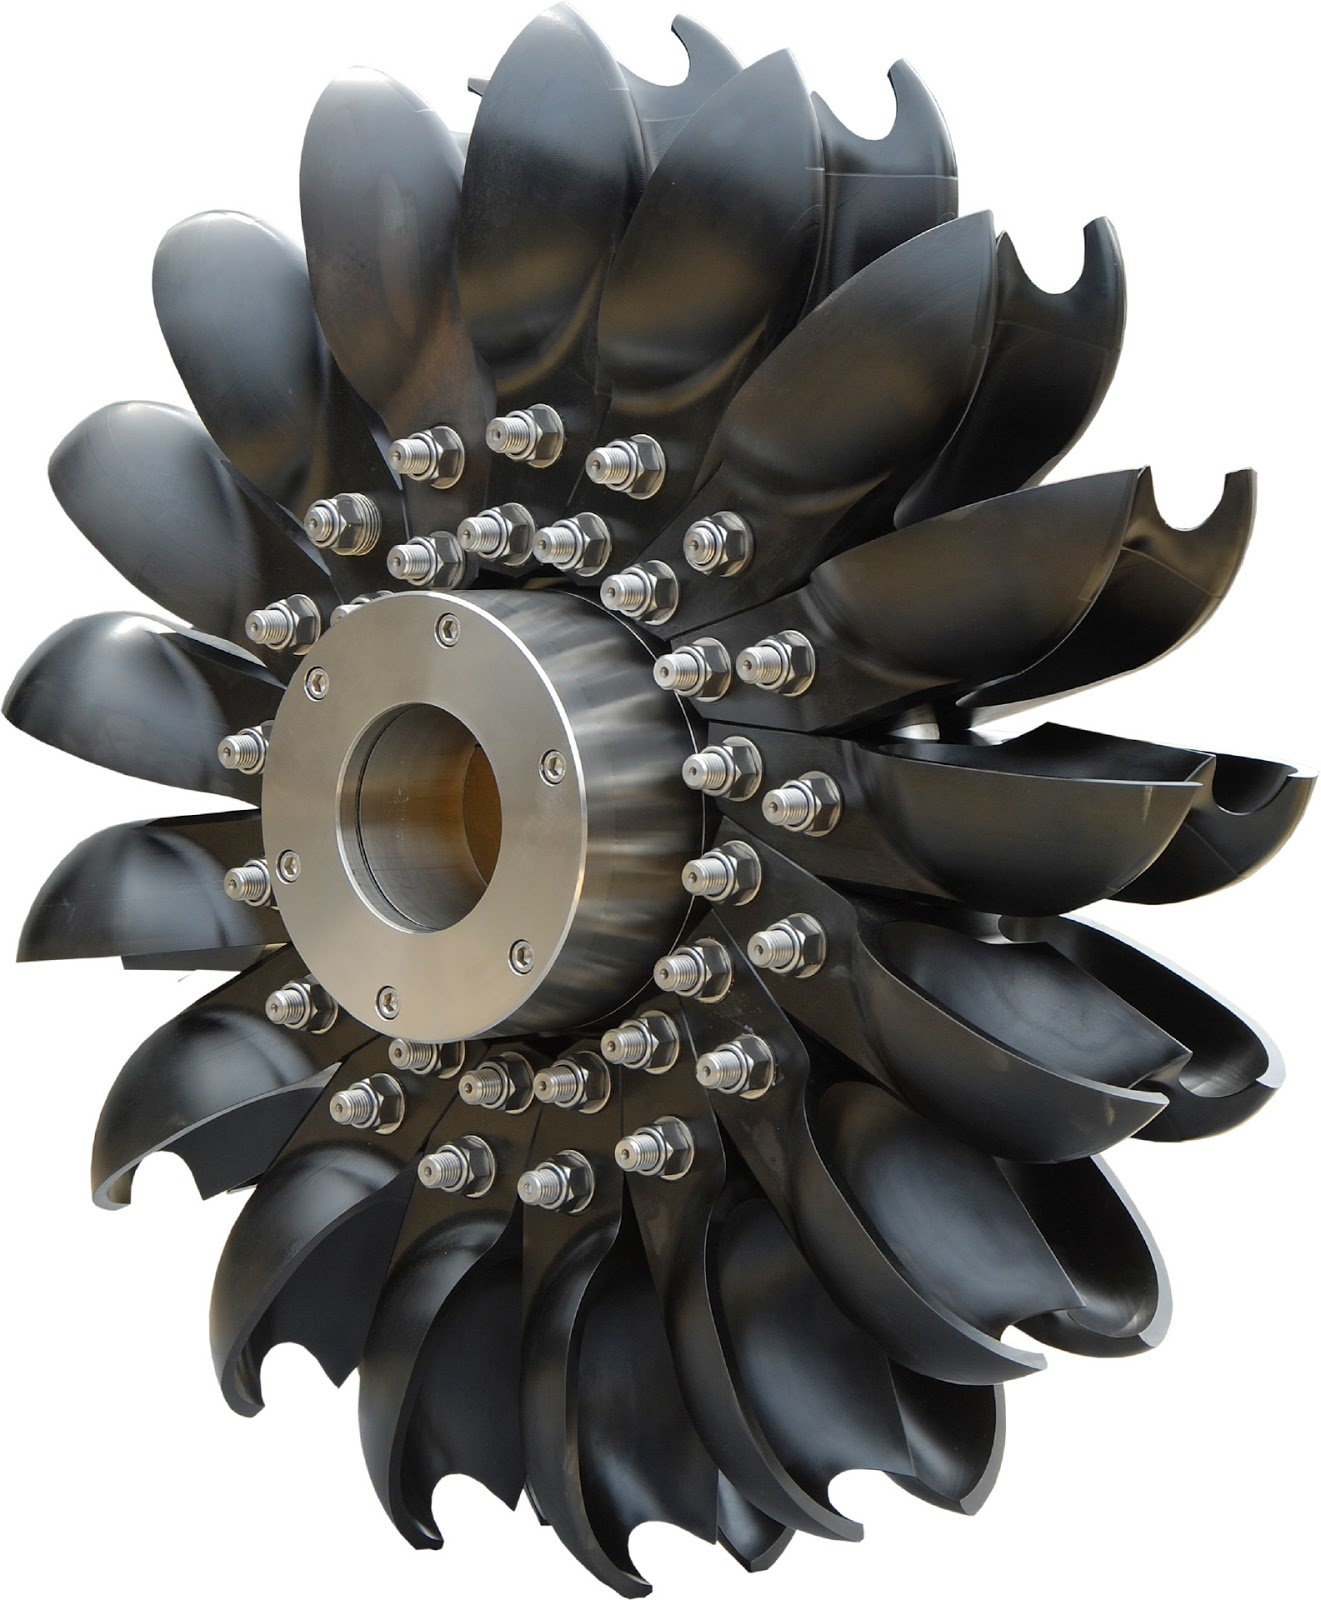
\includegraphics[height=5cm]{HydroAndWindPower/Figures/Pelton_Turbine_1.jpg}
		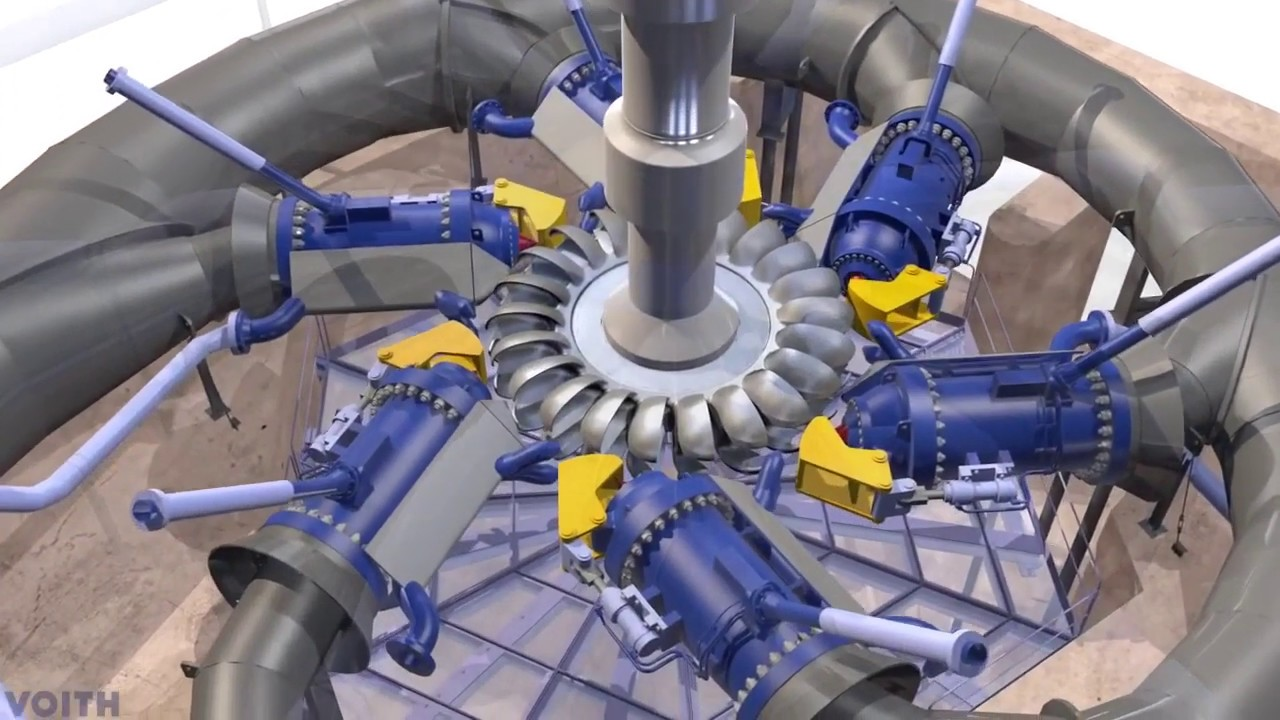
\includegraphics[height=5cm]{HydroAndWindPower/Figures/Pelton_Turbine_2.jpg}
	\caption{Left: a free Pelton wheel (runner), right: a built-in Pelton wheel driven by six water jets.}
	\label{Fig:pelton_turbine}
\end{figure}

For moderate heads ($50\,\mathrm{m}<H<500\,\mathrm{m}$) and low to high flow rates, Francis turbines are good solutions, see a runner in Fig.\,\ref{Fig:francis_turbine} left. Francis turbines are the first hydraulic turbines with radial inflow. It was designed by the American scientist James Francis. Francis turbine is a reaction turbine where the major part of pressure drop occurs in the turbine itself, unlike the impulse turbine where complete pressure drop takes place up to the entry point. The water flow completely fills the turbine passage during the operation. Francis turbines are generally installed with a vertical axis. Water enters the turbine through a spiral casing (see Fig.\,\ref{Fig:francis_turbine} middle) surrounding the guide vanes (magnified in Fig.\,\ref{Fig:francis_turbine} right). The water loses a part of its pressure in the volute (spiral casing) to maintain its speed. Then the water passes through the guide vanes where it is directed to strike the blades on the runner at an optimum angle. As the water flows through the runner, its pressure and angular momentum reduce. This reduction imparts reaction on the runner and power is transferred to the turbine shaft.

\begin{figure}[ht!]
	\centering
		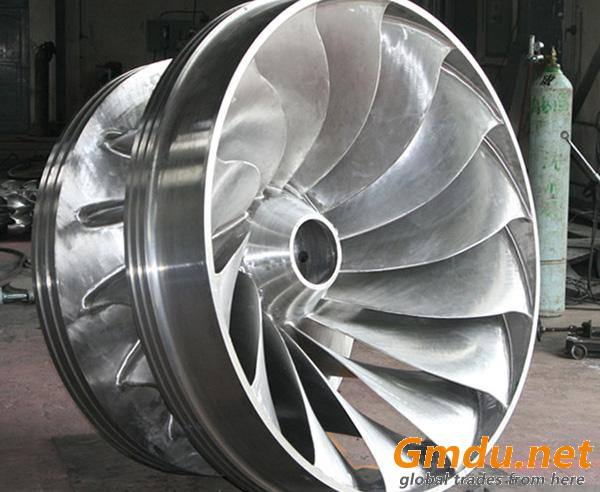
\includegraphics[height=4cm]{HydroAndWindPower/Figures/Francis_Turbine_1.jpg}
		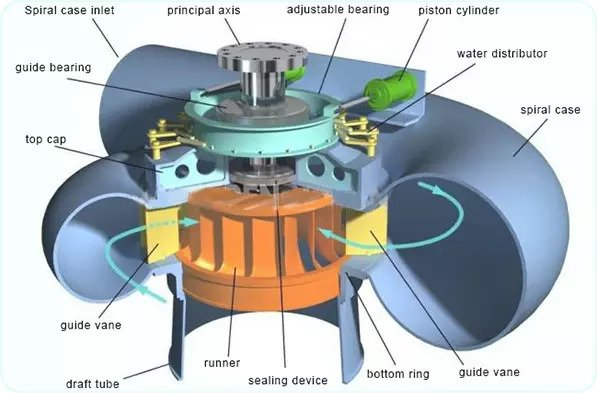
\includegraphics[height=4cm]{HydroAndWindPower/Figures/Francis_Turbine_2.jpg}
		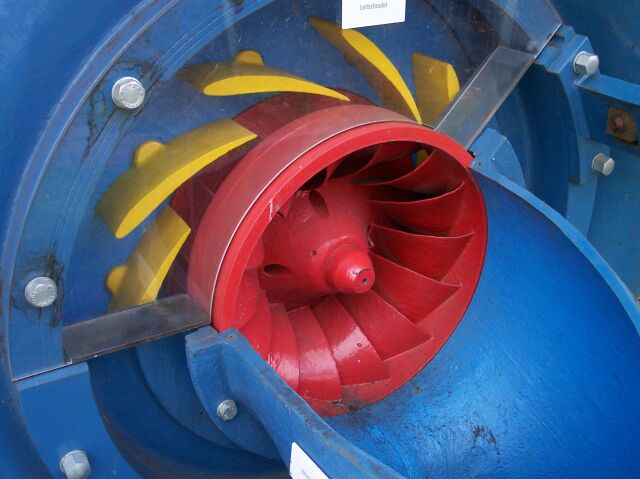
\includegraphics[height=4cm]{HydroAndWindPower/Figures/Francis_Turbine_3.jpg}
	\caption{Left: a free Francis wheel (runner), middle: a built-in Francis turbine into a spiral casing, right: magnified guide vanes.}
	\label{Fig:francis_turbine}
\end{figure}

For very low heads $H<50\,\mathrm{m}$ and a wide range of flow rates the optimal choice is the Kaplan turbine or one of its variant developed by the Austrian professor Viktor Kaplan in 1913. A runner of a Kaplan turbine is depicted in the left-hand side of Fig.\,\ref{Fig:kaplan_turbine}. Kaplan turbines are also reaction turbine and work similarly as Francis turbines. In fact, it is evolved from the Francis turbine and often referred to as propeller turbine. It also has a spiral casing and automatically adjusted propeller blades with automatically adjusted guide vanes (see Fig.\,\ref{Fig:kaplan_turbine} right) to achieve efficiency over a wide range of flow and water level. The main difference is that the water flows axially through the turbine instead of radially. It is capable of working at low head and high flow rates very efficiently, which is impossible with Francis turbines.

\begin{figure}[ht!]
	\centering
		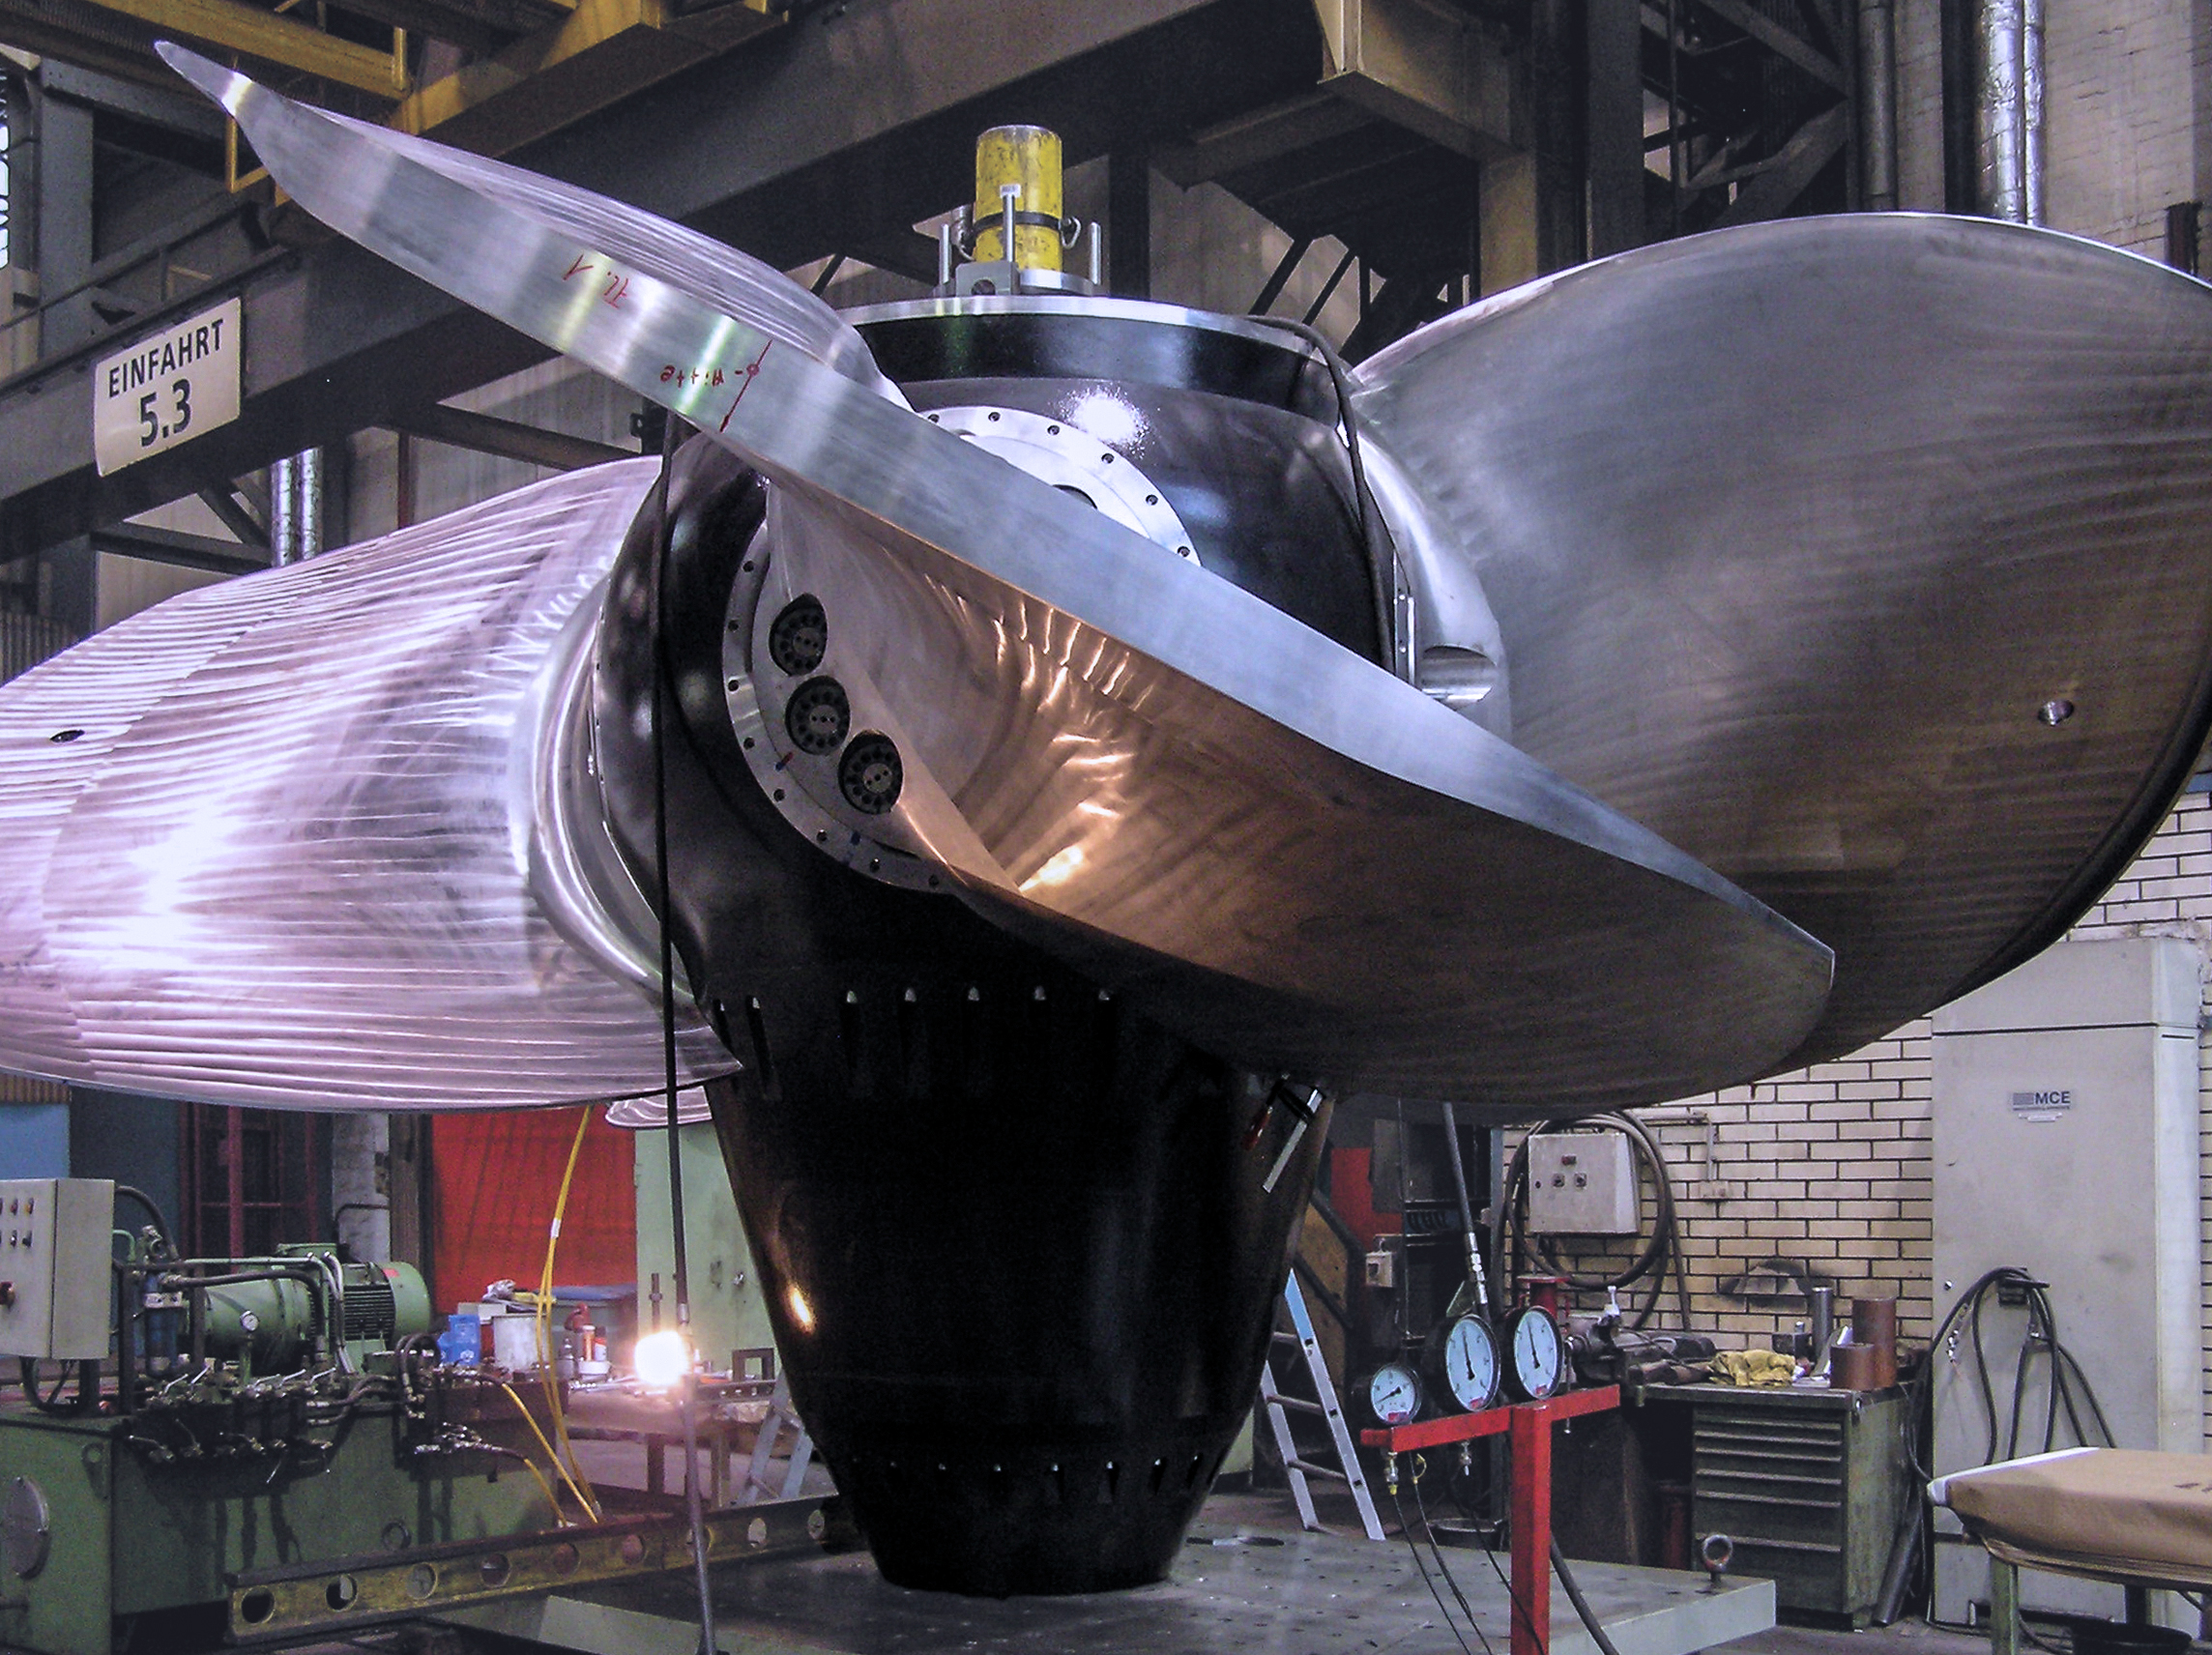
\includegraphics[height=5cm]{HydroAndWindPower/Figures/Kaplan_Turbine_1.jpg}
		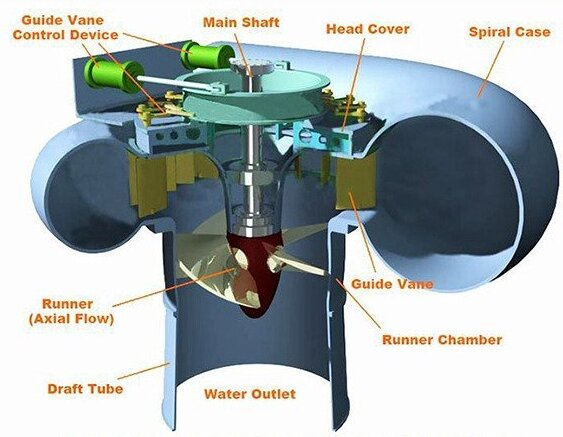
\includegraphics[height=5cm]{HydroAndWindPower/Figures/Kaplan_Turbine_3.jpg}
	\caption{Left: a free Kaplan wheel (runner), right: a built-in Kaplan wheel into a spiral casing with guide vanes (yellow).}
	\label{Fig:kaplan_turbine}
\end{figure}

The last type of turbines discussed here is the crossflow turbines useful in smaller hydroelectric sites ($5-100\,\mathrm{kW}$). Sometimes it is known as Banki-Mitchell or Ossberger turbines (depending on the country). These turbines are useful for a broad range of hydraulic heads ($1.75\,\mathrm{m}<H<200\,\mathrm{m}$); however, crossflow turbines are usually chosen for heads below $40\,\mathrm{m}$. Similarly, as the Pelton turbines, they are also impulsed turbines as they get energy from water by reducing the velocity, while the pressure stays nearly the same. Although one benefit of these turbines is the less complicated maintenance to keep them working, other turbines are likely more efficient and useful for large-scale applications. Therefore, it is seldom used in large hydropower projects. Figure\,\ref{Fig:crossflow_turbine} summarizes the runner (a cylindrical mechanism composed of blades arranged into a water wheel shape), the operation principle and an exploded figure of a crossflow turbine instalment in the left, middle and right panels, respectively.

\begin{figure}[ht!]
	\centering
		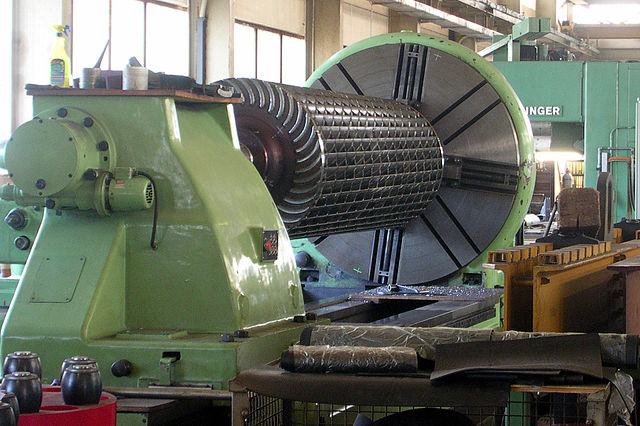
\includegraphics[height=4cm]{HydroAndWindPower/Figures/CrossFlow_Turbine_1.jpg}
		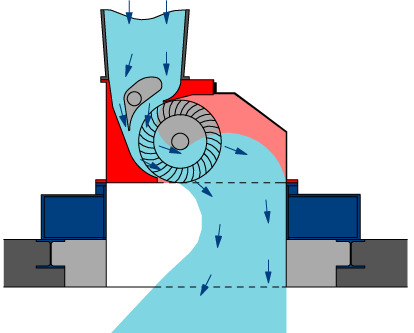
\includegraphics[height=4cm]{HydroAndWindPower/Figures/CrossFlow_Turbine_2.jpg}
		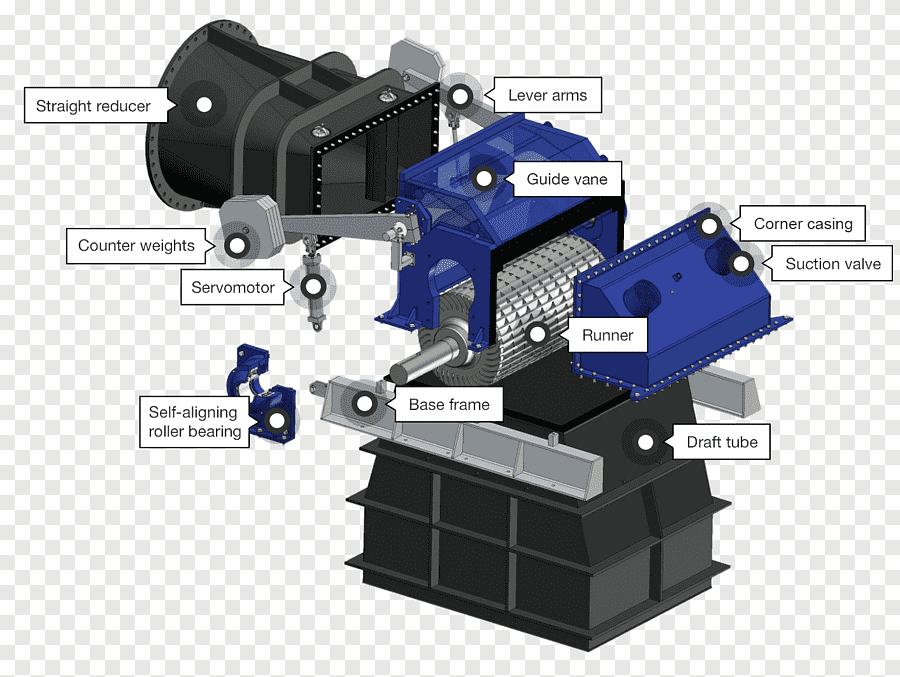
\includegraphics[height=4cm]{HydroAndWindPower/Figures/CrossFlow_Turbine_3.png}
	\caption{Left: a free crossflow wheel (runner), middle: operation principle, right: exploded figure of an instalment.}
	\label{Fig:crossflow_turbine}
\end{figure}

Figure\,\ref{Fig:water_turbines_application_chart} shows the range of application in term of the head $H$ and flow rate $Q$ of the different water turbines discussed above. It is worth noting that the diagonal turbine (e.g., the Deriaz turbine) is somewhere between the Francis (radial) and Kaplan (axial) turbines. That is, the flow in a diagonal turbine does not follow a full axial nor radial direction, but it is a diagonal mixture of the two. Like the Kaplan turbines, they also have adjustable runner blades and guide vanes. The bulb turbine is a variation of the propeller-type turbine (Kaplan turbine). In the bulb turbine arrangement, the generator is encapsulated and sealed within a streamlined watertight steel housing mounted in the centre of the water passageway. Due to the logarithmic scale of the head $H$ and the flow rate $Q$, the isolines of the power $P \propto QH$ are diagonal straight lines with a negative tangent. Keep in mind that such a chart depends on the manufacturer, the one presented in Fig.\,\ref{Fig:water_turbines_application_chart} is for demonstration purposes only.

\begin{figure}[ht!]
	\centering
		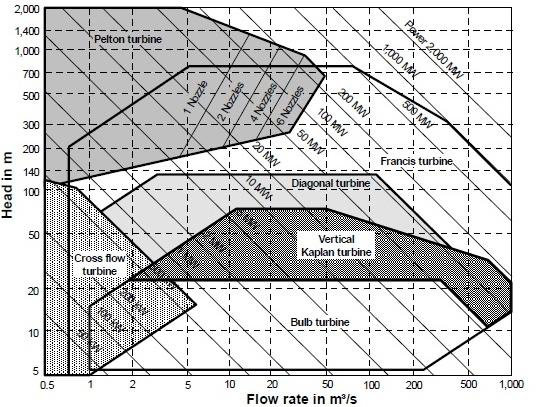
\includegraphics[width=10cm]{HydroAndWindPower/Figures/Water_Turbine_Chart.png}
	\caption{Application chart of water turbines as a function of the head $H$ and flow rate $Q$.}
	\label{Fig:water_turbines_application_chart}
\end{figure}

The application chart presented in Fig.\,\ref{Fig:water_turbines_application_chart} is a ``mess'' in the sense that clear trends can hard to be observed. In case of pumps, the specific speed defines the shape of the impellers; thus, it is a suitable quantity to characterise the types of the pumps, see again Sec.\,\ref{sec:dimensionless_numbers} and Fig.\,\ref{fig:nq} therein. Similarly, a specific speed can also be defined for water turbines as
%
\begin{equation}
n_q = n \frac{Q_{opt}^{1/2}}{H_{opt}^{3/4}},
\end{equation}
%
where $n$ is the revolution number in unit of $\mathrm{rpm}$, $Q_{opt}$ (in unit of $\mathrm{m^3/s}$) and $H_{opt}$ (in unit of $\mathrm{m}$) are the flow rate and the head at the best efficiency point. The specific speed can be reformulated with the usage of useful $P_u$ or input power $P_i$ since the flow rate is proportional to $Q \propto P_u/H \propto P_i/H$. In this way, the following definitions are also used in many textbooks:
%
\begin{align}
n_{\omega} &= \omega \frac{P_{u,opt}^{1/2}}{H_{opt}^{5/4}}, \\
n_s        &= n \frac{P_{i,opt}^{1/2}}{H_{opt}^{5/4}}.
\end{align}
%
With the usage of specific speed, the types of the different water turbines in the application chart shows a very clear trend, see Fig.\,\ref{Fig:water_turbines_application_chart_specific_speed}. With increasing specific speed, the tendency of the optimal choice of turbine type is Pelton, Francis and Kaplan. A similar clear tendency is displayed in terms of the head as well.

\begin{figure}[ht!]
	\centering
		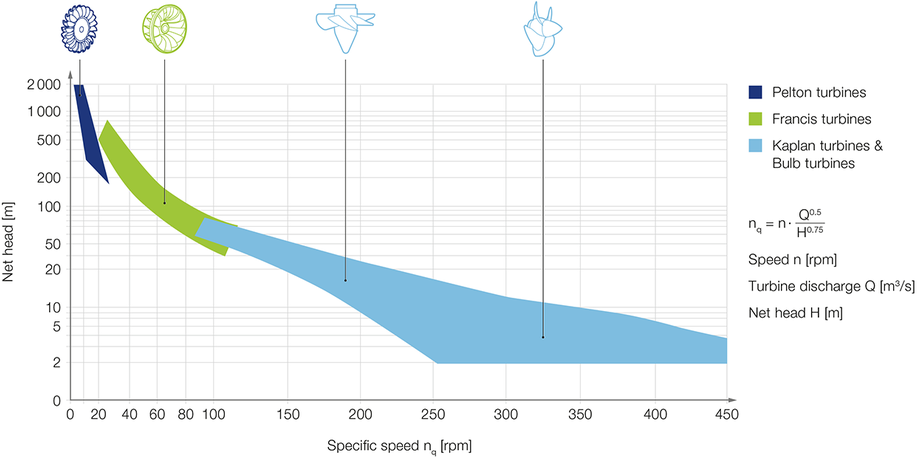
\includegraphics[width=12cm]{HydroAndWindPower/Figures/Water_Turbine_Chart_Specific_Speed.png}
	\caption{Application chart of water turbines as a function of the specific speed $n_q$.}
	\label{Fig:water_turbines_application_chart_specific_speed}
\end{figure}

%------------------------------------------------
\subsection{Characteristic curves of water turbines}
The fundamental equation of hydropower turbines as fluid machinery is the Euler equation. Similarly, as in the case of pumps, the theoretical specific work that can be extracted is possible via the change of the angular momentum of the fluid flow:
%
\begin{equation} \label{euler_equation_water_turbines}
H_{th} = \frac{c_{1u} u_1 - c_{2u} u_2}{g},
\end{equation}
%
where $u_1$ and $u_2$ are the circumferential velocities of the inlet and outlet points at the blades, respectively. The absolute velocity components parallel to the circumferential velocities are $c_{1u}$ and $c_{2u}$. Remember that the equivalent Euler equation for pumps can be found in Sec.\,\ref{sec:velocity_triangles_pumps} as Eq.\,\ref{radial_head}. The discharge (outlet) angular momentum is proportional to $c_{2u}$; thus, it is preferably zero. Any positive value of $c_{2u}$ is realised as energy loss at discharge (unextracted energy). In addition, for positive energy production, $c_{1u}>c_{2u}$ is necessary. For the Francis and Kaplan turbines, the optimal values of $c_{1u}$ is set by the guide vanes, see Figs.\,\ref{Fig:francis_turbine} and \ref{Fig:kaplan_turbine} again. The velocity components in Eq.\,\ref{euler_equation_water_turbines} depends primarily on the geometry of the turbine and its blades; therefore, they can be determined from the velocity triangles, see also Sec.\,\ref{sec:velocity_triangles_pumps}. In the case of the three widely used turbine types, they are summarised in Fig.\,\ref{Fig:velocity_triangles_water_turbines}: Pelton (top-left), Francis (top-right) and Kaplan (bottom). Observe that in this figure, for the Kaplan turbine, the index of the inlet and outlet are $2$ and $3$, respectively; however, throughout the text, we shall still use the conventional $1$ (inlet) and $2$ (outlet) indices. Note that even though the Pelton turbine is an impulse turbine, the Euler turbine equation is still valid.

\begin{figure}[ht!]
	\centering
		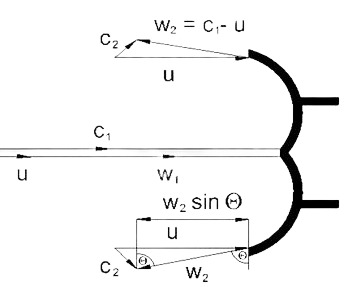
\includegraphics[height=4cm]{HydroAndWindPower/Figures/Velocity_Triangle_Pelton_Turbine.jpg}
		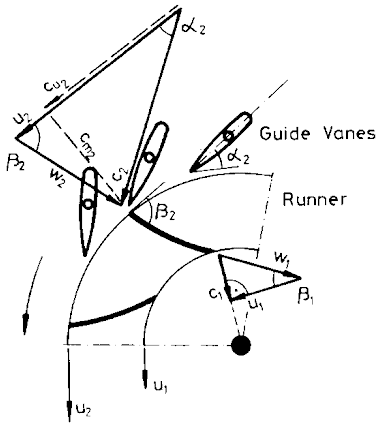
\includegraphics[height=5.5cm]{HydroAndWindPower/Figures/Velocity_Triangle_Francis_Turbine.png}
		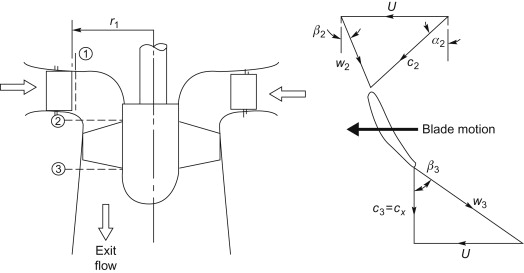
\includegraphics[height=5cm]{HydroAndWindPower/Figures/Velocity_Triangle_Kaplan_Turbine.jpg}
	\caption{Velocity triangles of the Pelton (top-left), Francis (top-right) and Kaplan (bottom) turbines.}
	\label{Fig:velocity_triangles_water_turbines}
\end{figure}

The Euler turbine equation is a good starting point to analyse the performance of a turbine. Nevertheless, as in the case of pumps, the real characteristic curves can be determined only via measurements due to the complicated flow conditions inside the runner. It customary to provide the flow rate $Q$, input hydraulic power $P_i$, overall efficiency $\eta_o$ and sometimes the torque $M$ as a function of the revolution number $n$ as characteristic curves with constant head $H$ and gate opening $GO$. For better comparison, quantities are usually specified to $H=1$ (unit head) and $D=1$ (unit runner diameter). The main reason is that the velocity triangles under the working conditions and unit quantities are geometrically similar, and the efficiency of the turbine remains unaffected. To determine the dimensionless unit flow rate, consider the following proportionality relationship:
%
\begin{equation} \label{derivation_of_unit_flow_rate}
Q = A_{ref} \cdot v_{ref} = \frac{D^2 \pi}{4} \sqrt{2gH} \propto D^2 H^{1/2},
\end{equation}
%
where the fluid flow with reference velocity $\sqrt{2gH}$ has the same kinetic energy as the potential energy of a steady water column with height $H$. Observe that the constants in the last term of Eq.\,\eqref{derivation_of_unit_flow_rate} can be eliminated since between the last two terms there is a proportionality relation. Taking the ratio of the first and the last terms in Eq.\,\eqref{derivation_of_unit_flow_rate}, the unit flow rate can be defined as
%
\begin{equation}
Q_U = Q_{11} = \frac{Q}{D^2 H^{1/2}}.
\end{equation}
%
In a similar way, the unit revolution number is derived as
%
\begin{align}
u = D \pi n &\propto v_{ref} = \sqrt{2gH}, \\
D \pi n &\propto H^{1/2}, \\
n_U = n_{11} &= \frac{nD}{H^{1/2}}.
\end{align}
%
Also, the unit input power:
%
\begin{align}
P_i &= Q \rho g H \propto D^2 H^{1/2} H = D^2 H^{3/2}, \\
P_U &= P_{11} = \frac{P_i}{D^2 H^{3/2}},
\end{align}
%
where the proportionality relationship $Q \propto D^2 H^{1/2}$ from Eq.\,\ref{derivation_of_unit_flow_rate} is exploited. Finally, the unit torque:
%
\begin{align}
M &\propto \frac{P_i}{\omega} \propto \frac{P_i}{n} \propto \frac{D^2 H^{3/2}}{H^{1/2}/D}, \\
M_U &= M_{11} = \frac{M}{D^3 H}.
\end{align}
%
It is important to emphasize that if a liquid differs from water (e.g., the flow rate at the final stage of a process in a chemical application is exploited to produce electricity), the density cannot be omitted as a constant during the derivations of the unit quantities. The ``nature'' of the characteristic curves of the Pelton (left), Kaplan (middle) and Francis (right) turbines are shown in Fig.\,\ref{Fig:typical_characteristic_curves_of_water_turbines} with constant head $H$ and at different gate opening $GO$ values in percentage.

\begin{figure}[ht!]
	\centering
		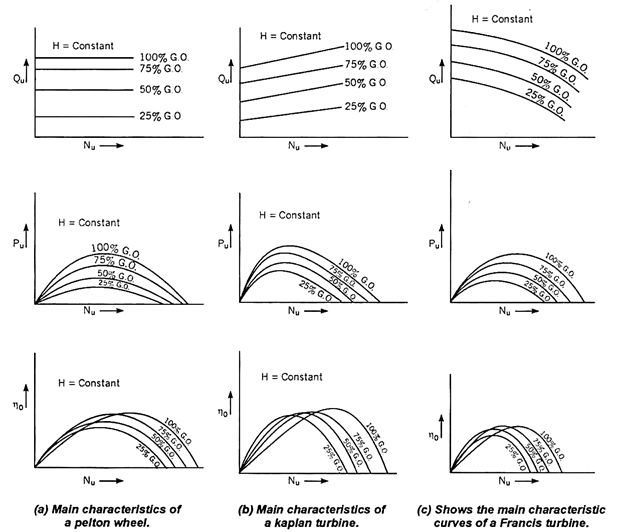
\includegraphics[width=14cm]{HydroAndWindPower/Figures/Characteristic_Curves_All_Types.png}
	\caption{Typical characteristic curves of the Pelton (left), Kaplan (middle) and Francis (right) turbines.}
	\label{Fig:typical_characteristic_curves_of_water_turbines}
\end{figure}

In order to determine the optimal operation conditions (e.g., $H_{opt}$ or $Q_{opt}$), for instance, to calculate the specific speed of the turbine, it is useful to present the constant efficiency isolines in the characteristic curve diagrams. An example is shown in the top panel of Fig.\,\ref{Fig:hill_chart_and_best_efficiency}, where such a representation is often referred to as efficiency hill chart. As a local maximum, the best efficiency point can be estimated. The characteristics of the maximum achievable efficiencies are presented in the bottom panel of Fig.\,\ref{Fig:hill_chart_and_best_efficiency} for different turbine types. Keep in mind that the Deriaz turbine is halfway between the Kaplan and the Francis turbines. From this diagram, it is sharply visible, that for different specific speeds $n_s$, different turbine types are optimal. Observe that moving away from the best peak efficiency point, the maximum achievable efficiency decreases significantly. Since, roughly speaking, the specific speed $n_s$ or $n_q$ is inversely proportional to the head $H$ (see Fig.\,\ref{Fig:water_turbines_application_chart_specific_speed}), optimal selection of the turbines greatly depends on the available head of the hydropower plant.

\begin{figure}[ht!]
	\centering
		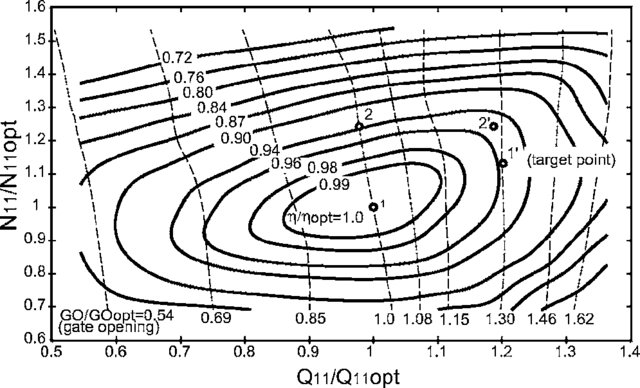
\includegraphics[width=10cm]{HydroAndWindPower/Figures/Efficiency_Hill.jpg}\\
		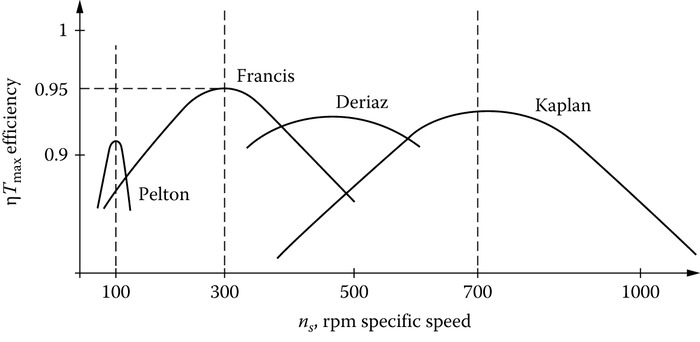
\includegraphics[width=11cm]{HydroAndWindPower/Figures/Efficiency_Of_Turbines.jpg}
	\caption{Typical characteristic curves of the Pelton (left), Kaplan (middle) and Francis (right) turbines.}
	\label{Fig:hill_chart_and_best_efficiency}
\end{figure}

%------------------------------------------------
\subsection{Final remarks}
Finally, let us discuss the current state of production and the further potential of hydroelectricity, and figure out how significant is its impact on global energy production. In 2018, the total installed capacity for electricity production is about $1260\,\mathrm{GW}$ ($948.8\,\mathrm{Mtoe}$, $1\,\mathrm{Mtoe}=11.63\,\mathrm{TWh}$). Here Mtoe stands for Million tonnes oil equivalent. In contrast, the total primary energy consumption (oil, natural gas, coal, nuclear energy, hydroelectricity, other renewables) of the world in 2018 was $18394\,\mathrm{GW}$ ($13846\,\mathrm{Mtoe}$). This translates to approximately a $14.6\%$ share of hydroelectricity from the total energy consumption of the world ($62.8\%$ from all renewables). Total global gross hydropower potential is estimated to be approximately $14000\,\mathrm{GW}$, if one assumes that the potential energy of all the rainfall has been exploited as it runs down to the sea level. Naturally, such an assumption is a huge overestimate; thus, the technical potential is about $3000\,\mathrm{GW}$, meaning that $40\%$ of the global energy consumption can be satisfied by hydropower plants in the near future. Keep in mind, however, that energy hunger of the countries increases as well.

Our conclusion can be more optimistic compared to wind power. The capacity of hydroelectricity is huge, and our consumption is huge as well; however, hydroelectricity will definitely play an important role worldwide. Compared to other renewable energy sources as wind and solar panels, the cost of energy production is the cheapest. The average cost in USD for $1\,\mathrm{kWh}$ electric energy are as follows; hydroelectricity: $0.047$, onshore wind $0.056$, offshore wind $0.127$, photovoltaic solar $0.085$ and concentrating solar $0.185$. Also, other factors have to be taken into account, such as the lifetime (duration of utilisation in years) of the instalments: offshore wind $5\,\mathrm{y}$, onshore wind $30\,\mathrm{y}$, solar $10-15\,\mathrm{y}$ and hydropower $150\,\mathrm{y}$. Thus, hydropower is a long-term investment with low maintenance cost for more than a century; it needs no rare metals as the photovoltaic modules and lacks the low power density of wind power. In Fig.\,\ref{Fig:global_hydropower_potential}, the theoretical potential is depicted in the left-hand side, and the planned hydropower projects are summarised in the right-hand side.

\begin{figure}[ht!]
	\centering
		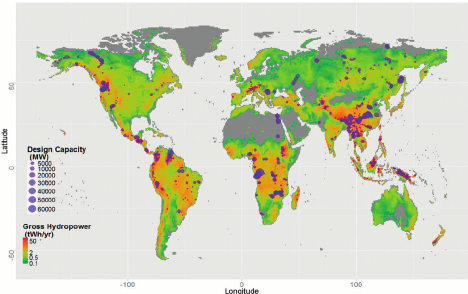
\includegraphics[height=4.6cm]{HydroAndWindPower/Figures/Global_Hydropower_Potential.png}
		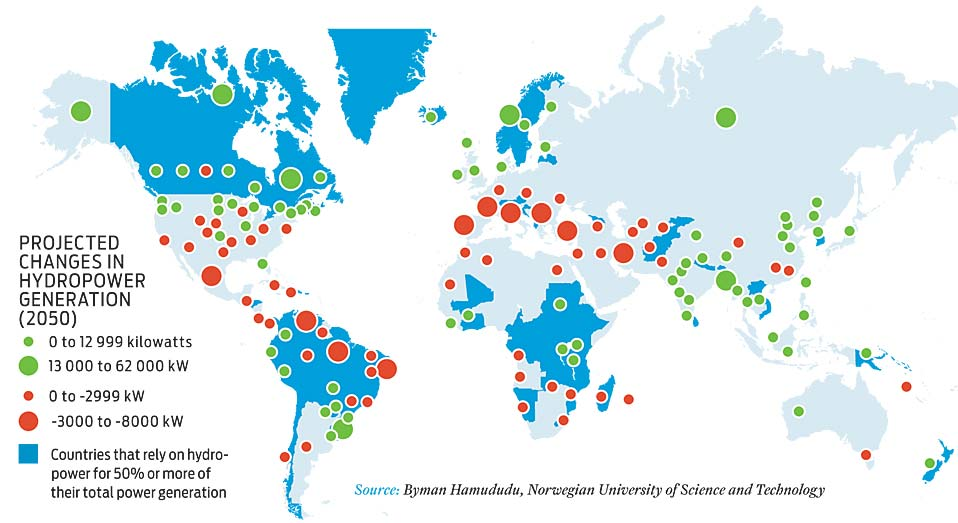
\includegraphics[height=4.6cm]{HydroAndWindPower/Figures/The_Future_Of_Hydropower.jpg}
	\caption{Theoretical potential of hydropower (left-hand side) and the planned hydropower projects (right-hand side).}
	\label{Fig:global_hydropower_potential}
\end{figure}

%------------------------------------------------
\section{Problems}

\noindent {\bf Problem \thesection.\theprob}\stepcounter{prob}

The cross-section of a plant water channel is given. The measured average water depth is $\overline{h}=2.9\,\mathrm{m}$, the width of the channel is $\overline{B}=25\,\mathrm{m}$. The velocity of the water flow is measured at several locations of the cross-section using a cup-type anemometer. The calculated average velocity is $\overline{v}=0.4\,\mathrm{m/s}$. The height difference between the upstream and downstream water depth at the dam is $h_{upstream}-h_{downstream}=4.5\,\mathrm{m}$. The efficiency of the turbine is $\eta_{turbine}=90\,\%$ the efficiency of the generator is $\eta_{generator}=96\,\%$. The input power and useful power of the power plant are to be calculated. What is the value of the hydraulic radius? What type of turbine is suitable for this power plant?

\noindent Solution:

\begin{itemize}
\item $A=\overline{h}\overline{B}=72.5\,\mathrm{m^2}$
\item $\overline{Q}=A\overline{v}=29\,\mathrm{m^3/s}$
\item $\overline{H}=h_{upstream}-h_{downstream}=4.5\,\mathrm{m}$
\item $\overline{P}_{input}=\overline{Q}\rho g\overline{H}=1.28\,\mathrm{MW}$
\item $\overline{P}_{useful}=\eta_{turbine}\eta_{generator}\overline{P}_{input}=1.106\,\mathrm{MW}$
\item $R_h=\frac{Area}{Perimeter}=\frac{\overline{B}\overline{h}}{2\overline{h}+\overline{B}}=2.35\,\mathrm{m}$
\end{itemize}

\noindent Turbine type: Kaplan turbine.

%%%%%%%%%%%%%%%%%%%%%%%%%%%%%%%%%%%%%%%%%%%%%%%%%%%%%%%%%%%%

\vspace{1cm}
\noindent {\bf Problem \thesection.\theprob}\stepcounter{prob}

The instantaneous efficiency of an existing wind turbine is to be calculated. The measured average wind speed at the level of the rotor is $\overline{v}_1=12\,\mathrm{m/s}$. The average speed of the air behind the rotor is $\overline{v}_3=8\,\mathrm{m/s}$. The diameter of the rotor is $D_2=55\,\mathrm{m}$, the density of the air is $\rho_{air}=1.2\,\mathrm{kg/m^3}$. Find the calculated efficiency related to the theoretical maximum of the efficiency?

\noindent Solution:

\begin{itemize}
\item $\Delta \overline{v}=\overline{v}_1-\overline{v}_3=4\,\mathrm{m/s}$
\item $A_2=\frac{D_2^2\pi}{4}=2376\,\mathrm{m^2}$
\item $\overline{P}_{input}=\rho_{air}A_2\overline{v}_1\frac{\overline{v}_1^2}{2}=2.463\,\mathrm{MW}$
\item $\overline{P}_{useful}=\rho_{air}A_2\overline{v}_1^3\left(1-\frac{\Delta \overline{v}}{2v_1}\right)^2\frac{\Delta \overline{v}}{v_1}=1.140\,\mathrm{MW}$
\item $\eta=C_P=\frac{\overline{P}_{useful}}{\overline{P}_{input}}=0.463<\frac{16}{27}=0.593$
\end{itemize}

%%%%%%%%%%%%%%%%%%%%%%%%%%%%%%%%%%%%%%%%%%%%%%%%%%%%

\vspace{1cm}
\noindent {\bf Problem \thesection.\theprob}\stepcounter{prob}

How large is the power of a wind turbine of $30 m$ rotor diameter if the wind speed is $8 m/s$? The Betz limit of the power coefficient $Cp$ is $0.593$.


\clearpage